% En este capítulo, se ha utilizado el sistema de calibración, compuesto por la placa desarrollada en el Capítulo \ref{cap:datalogger} y el software descrito en el Capítulo \ref{cap:aplicacionweb}, para realizar dos ensayos. 



% Inicialmente, se identificarán dos posiciones dentro del túnel de viento que presenten condiciones similares de flujo de aire para la medición de los anemómetros. Posteriormente, se detallarán dos ejemplos de calibración de anemómetros en el túnel de viento, utilizando el sistema mencionado.

En este capítulo se presentan los resultados de dos mediciones. La primera medición permite identificar dos posiciones dentro del túnel de viento donde se presentan condiciones similares de flujo de aire para la medición de los anemómetros. La segunda medición consiste en la realización de un presupuesto de incertidumbre para obtener la calibración de un anemómetro bajo prueba. Ambos ensayos se llevaron a cabo utilizando el sistema desarrollado y el túnel de viento. Para todas las mediciones se utilizo el sistema de referencia definido en la figura \ref{fig:sisReferenciaZmed}, donde el eje \textbf{z} se corresponde con el eje vertical, el eje \textbf{y} se corresponde con el eje longitudinal y el eje \textbf{x} se corresponde con el eje trasversal.

\begin{figure}[H]
    \centering
    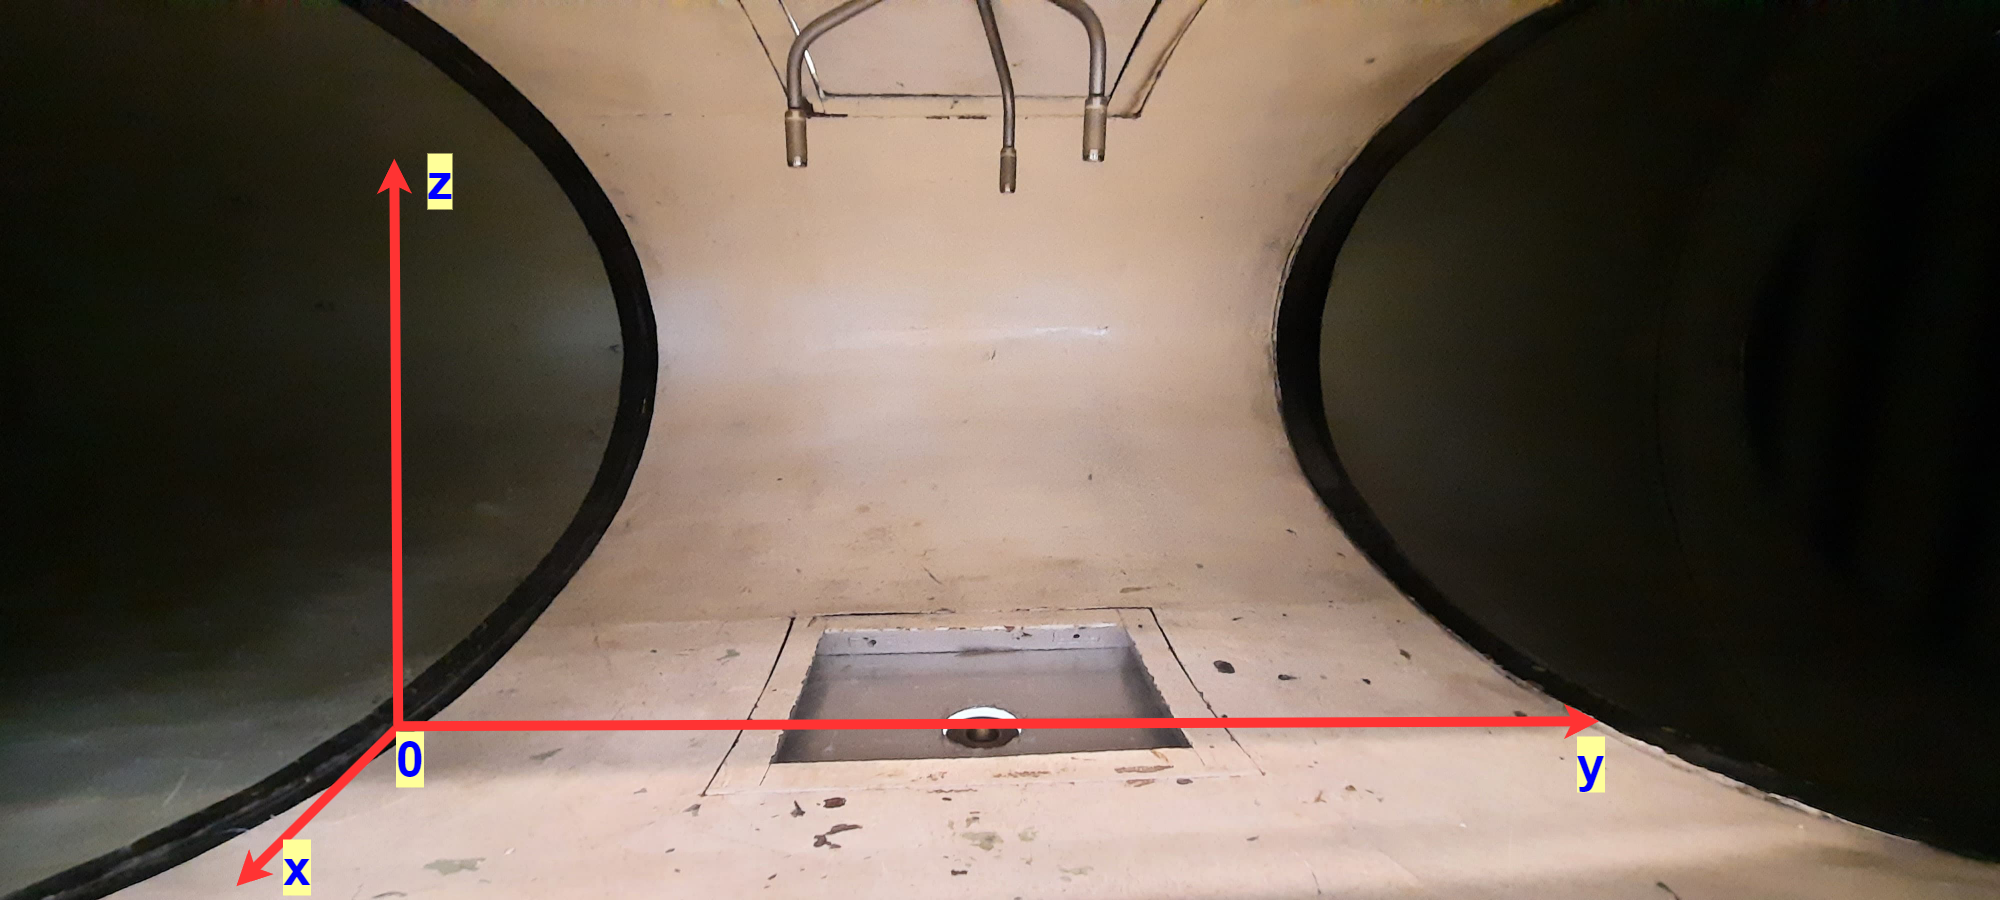
\includegraphics[width=0.9\linewidth]{Figuras/resultados/sisReferenciaZmed.png}
    \caption{Sistema de referencia utilizado para realizar las mediciones adentro del túnel de viento.}
    \label{fig:sisReferenciaZmed}
\end{figure}
%%%%%%%%%%%%%%%%%%%%%%%%%%%%%%%%%%%%%%%%%%%%%%%%%%%%%%%%%%%%%%%%%%%%%%%%%%%%%%%%%%%%%%%%%%%%%%%%%%%%%%%%%%%%%%%%%%%%%%%%
\section{Caracterización de la zona de medición}\label{sec:caracterZonaMed}
% terminar esta parte
El flujo de aire a lo largo, alto y profundo en toda la zona de medición no es constante debido a los cambios de sección presentes al principio y al final de dicha la zona, lo cual provoca variaciones en la dirección e  intensidad del viento. Para determinar dos posiciones donde el flujo de aire presenta la misma intensidad, una para el anemómetro patrón y otra para el anemómetro bajo calibración, se realizó un ensayo considerando las limitaciones de las dimensiones de los anemómetros dentro del volumen de medición. El objetivo del ensayo fue identificar dos posiciones en el espacio donde se mida la misma intensidad de viento. Para ello, se utilizó el sensor patrón Vaisala, modelo WMT700. Se simplificó el problema a una dimensión, manteniendo constante la altura del sensor en \SI{39.5}{\centi\meter} respecto a la base del túnel y centrando el sensor en el medio en la dirección trasversal, $x=0$. Solamente se varió el eje longitudinal desde \SI{-20}{\centi\meter} hasta \SI{60}{\centi\meter} en incrementos de \SI{10}{\centi\meter}. En cada posición, se configuró la aplicación web para medir y controlar la velocidad del aire en cinco valores: \SI{5}{\meter\per\second}, \SI{10}{\meter\per\second}, \SI{15}{\meter\per\second}, \SI{20}{\meter\per\second} y \SI{25}{\meter\per\second}. En la Figura \ref{fig:caracterPuntos} se muestra el sensor en tres posiciones específicas: a \SI{-20}{\centi\meter}, a \SI{20}{\centi\meter} y a \SI{60}{\centi\meter} respecto del origen del sistema de referencia ilustrado en la Figura \ref{fig:sisReferenciaZmed}.

\begin{figure}[H]
    \centering
    \begin{minipage}[b]{0.18\textwidth}
        \centering
        \subcaptionbox{\label{fig:-20cm}}{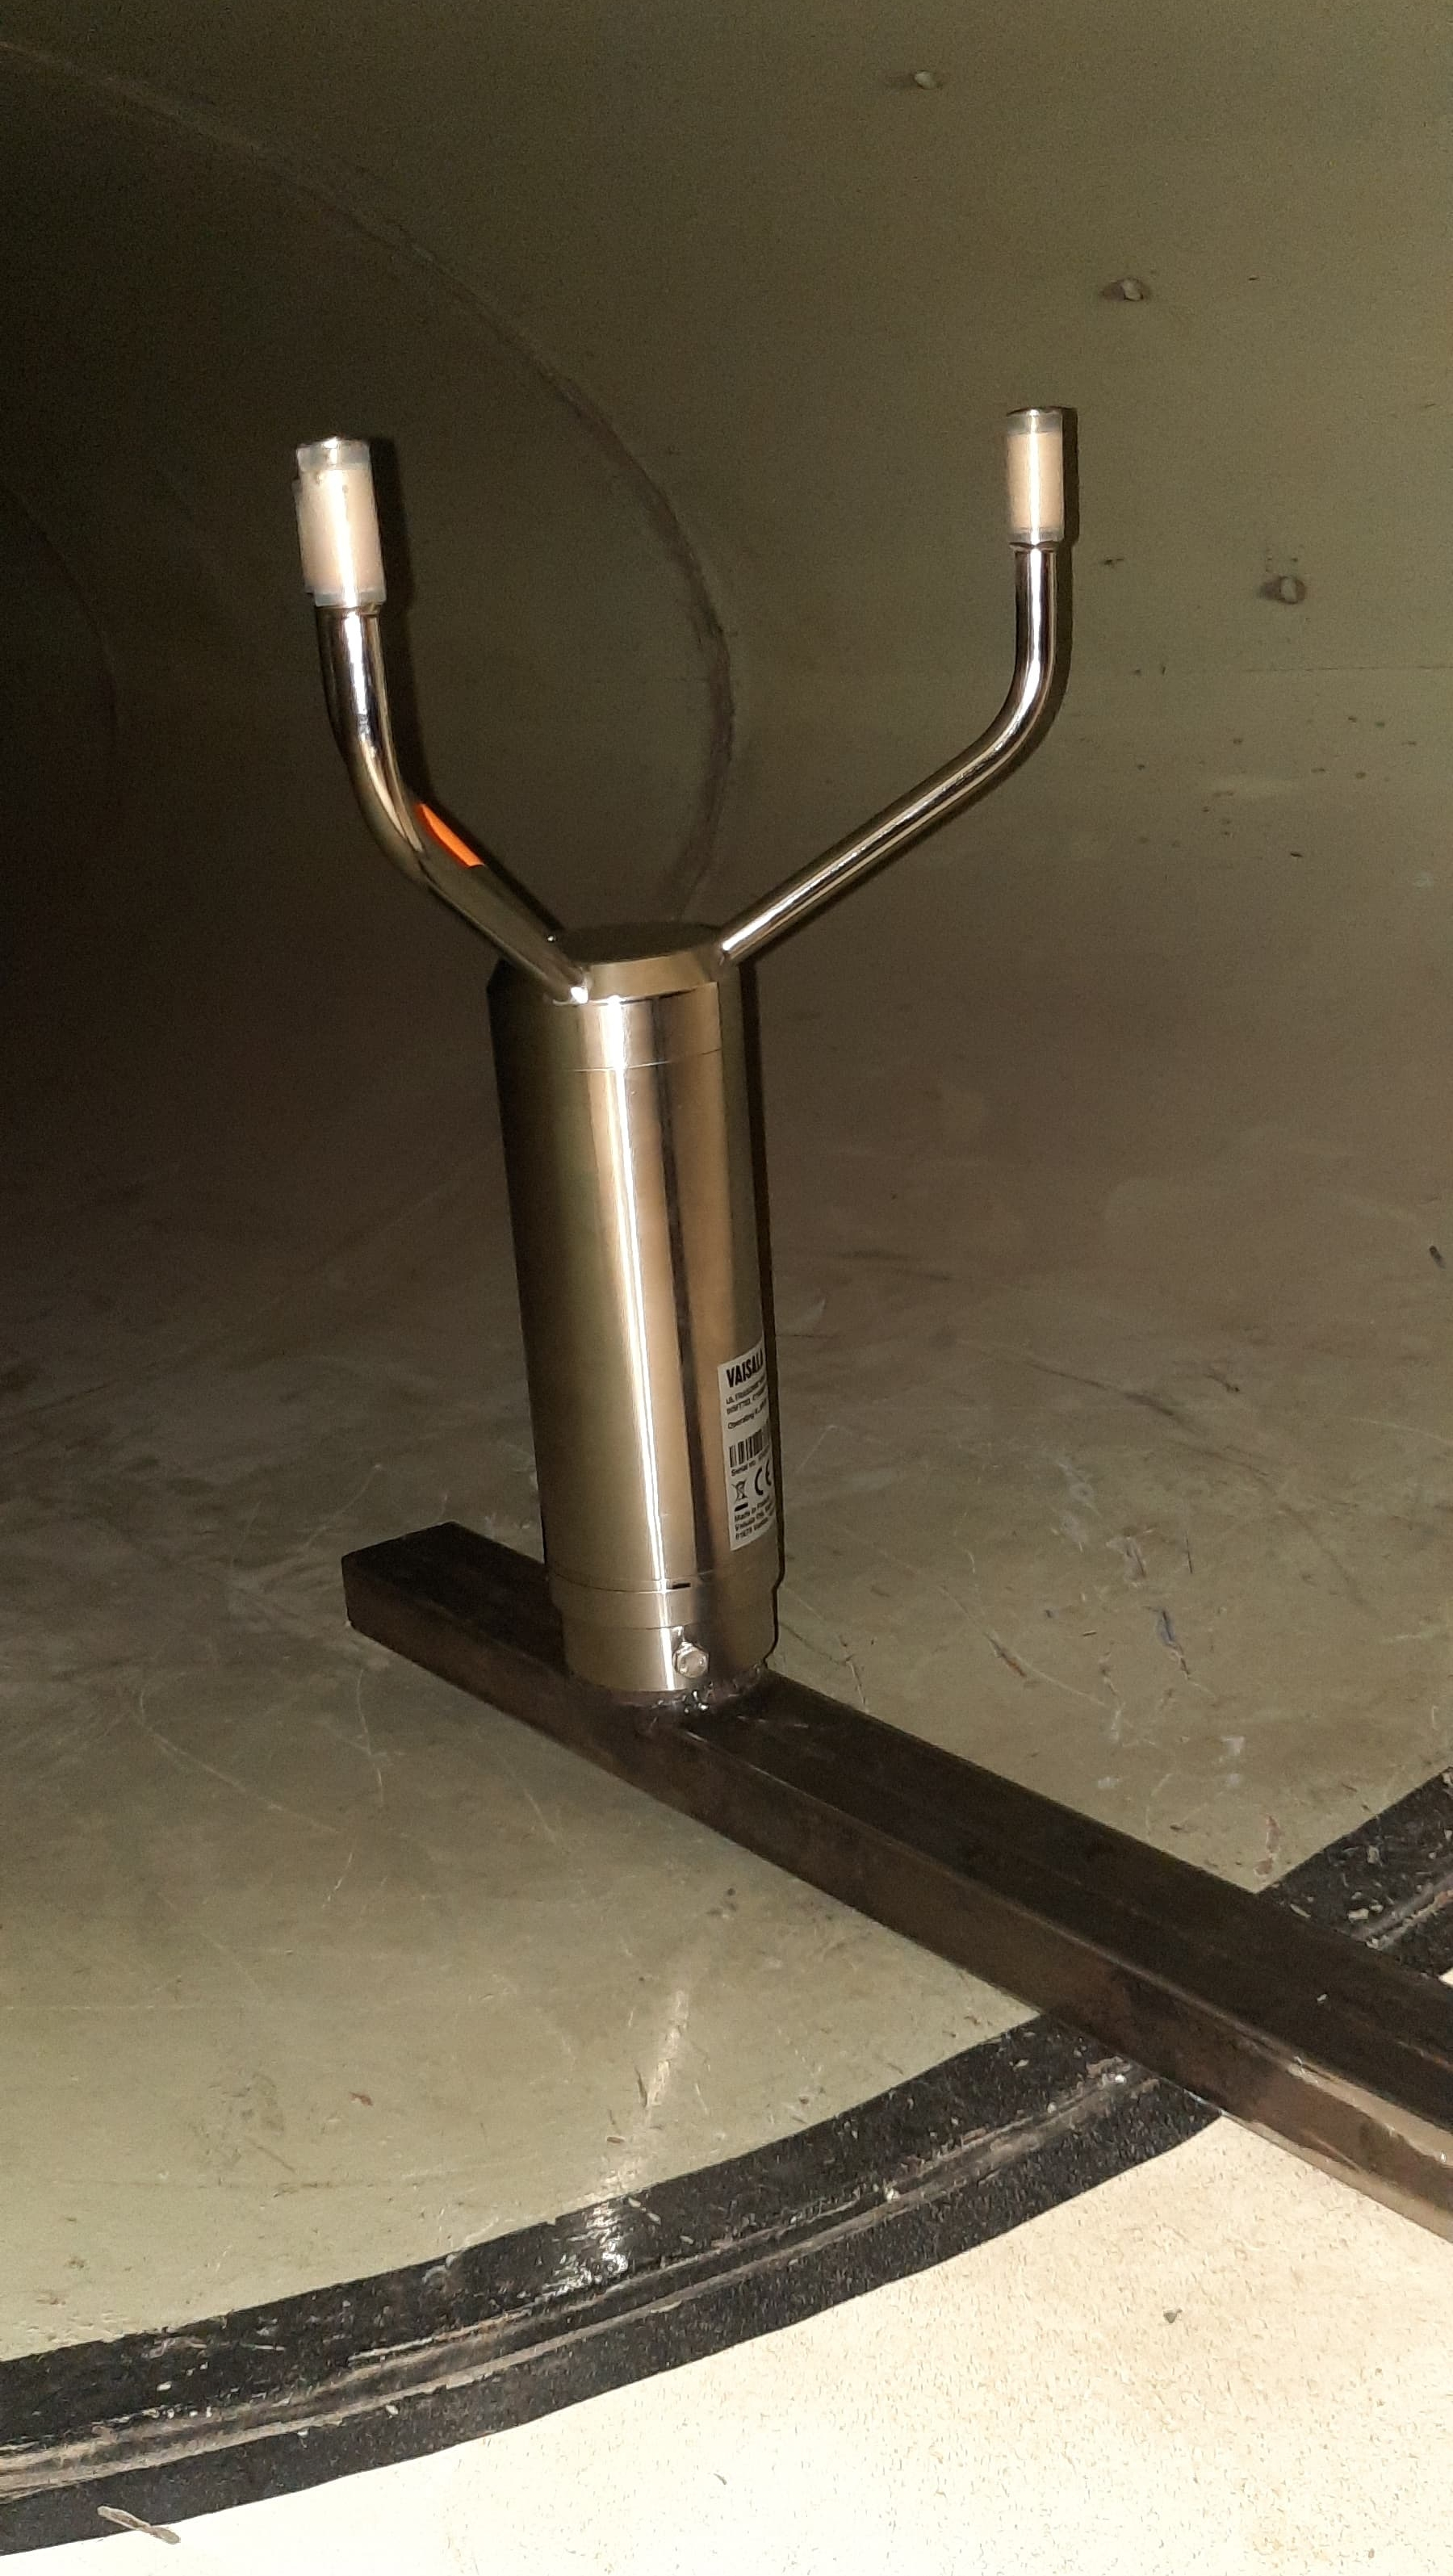
\includegraphics[width=\textwidth]{Figuras/resultados/caracterizacion/-20cm.jpg}}
    \end{minipage}%
    \hspace{2.5em} % Espacio horizontal entre las columnas
    \begin{minipage}[b]{0.33\textwidth}
        \centering
        \subcaptionbox{\label{fig:20cm}}{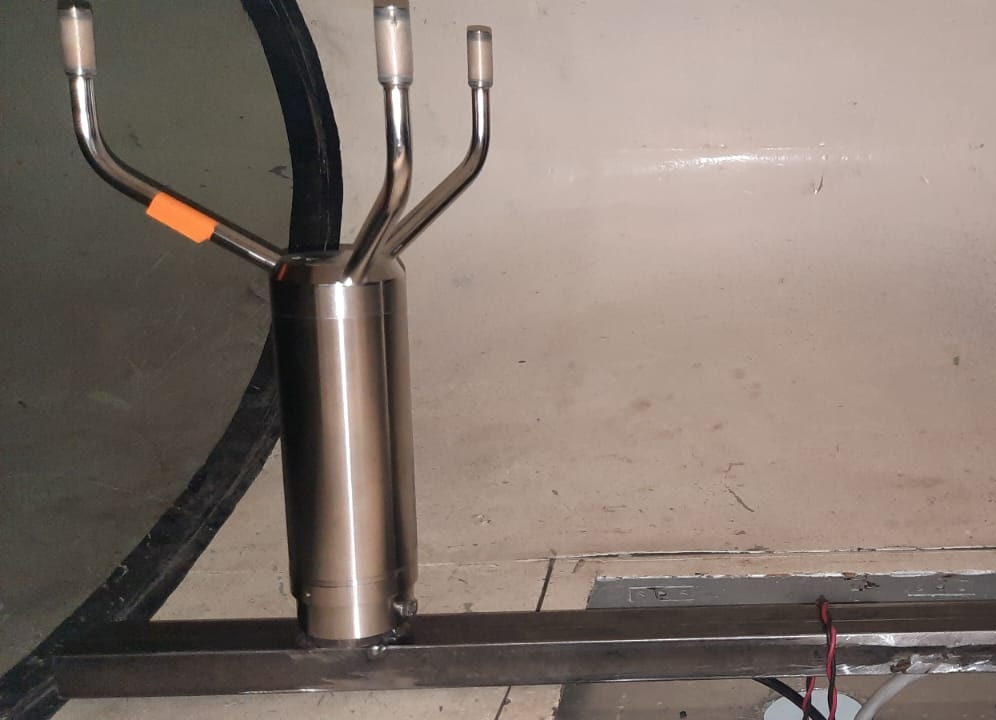
\includegraphics[width=\textwidth]{Figuras/resultados/caracterizacion/20cm.jpg}}
    \end{minipage}
    % \vspace{10em}
    \begin{minipage}[b]{0.5\textwidth}
        \centering
        \subcaptionbox{\label{fig:60cm}}{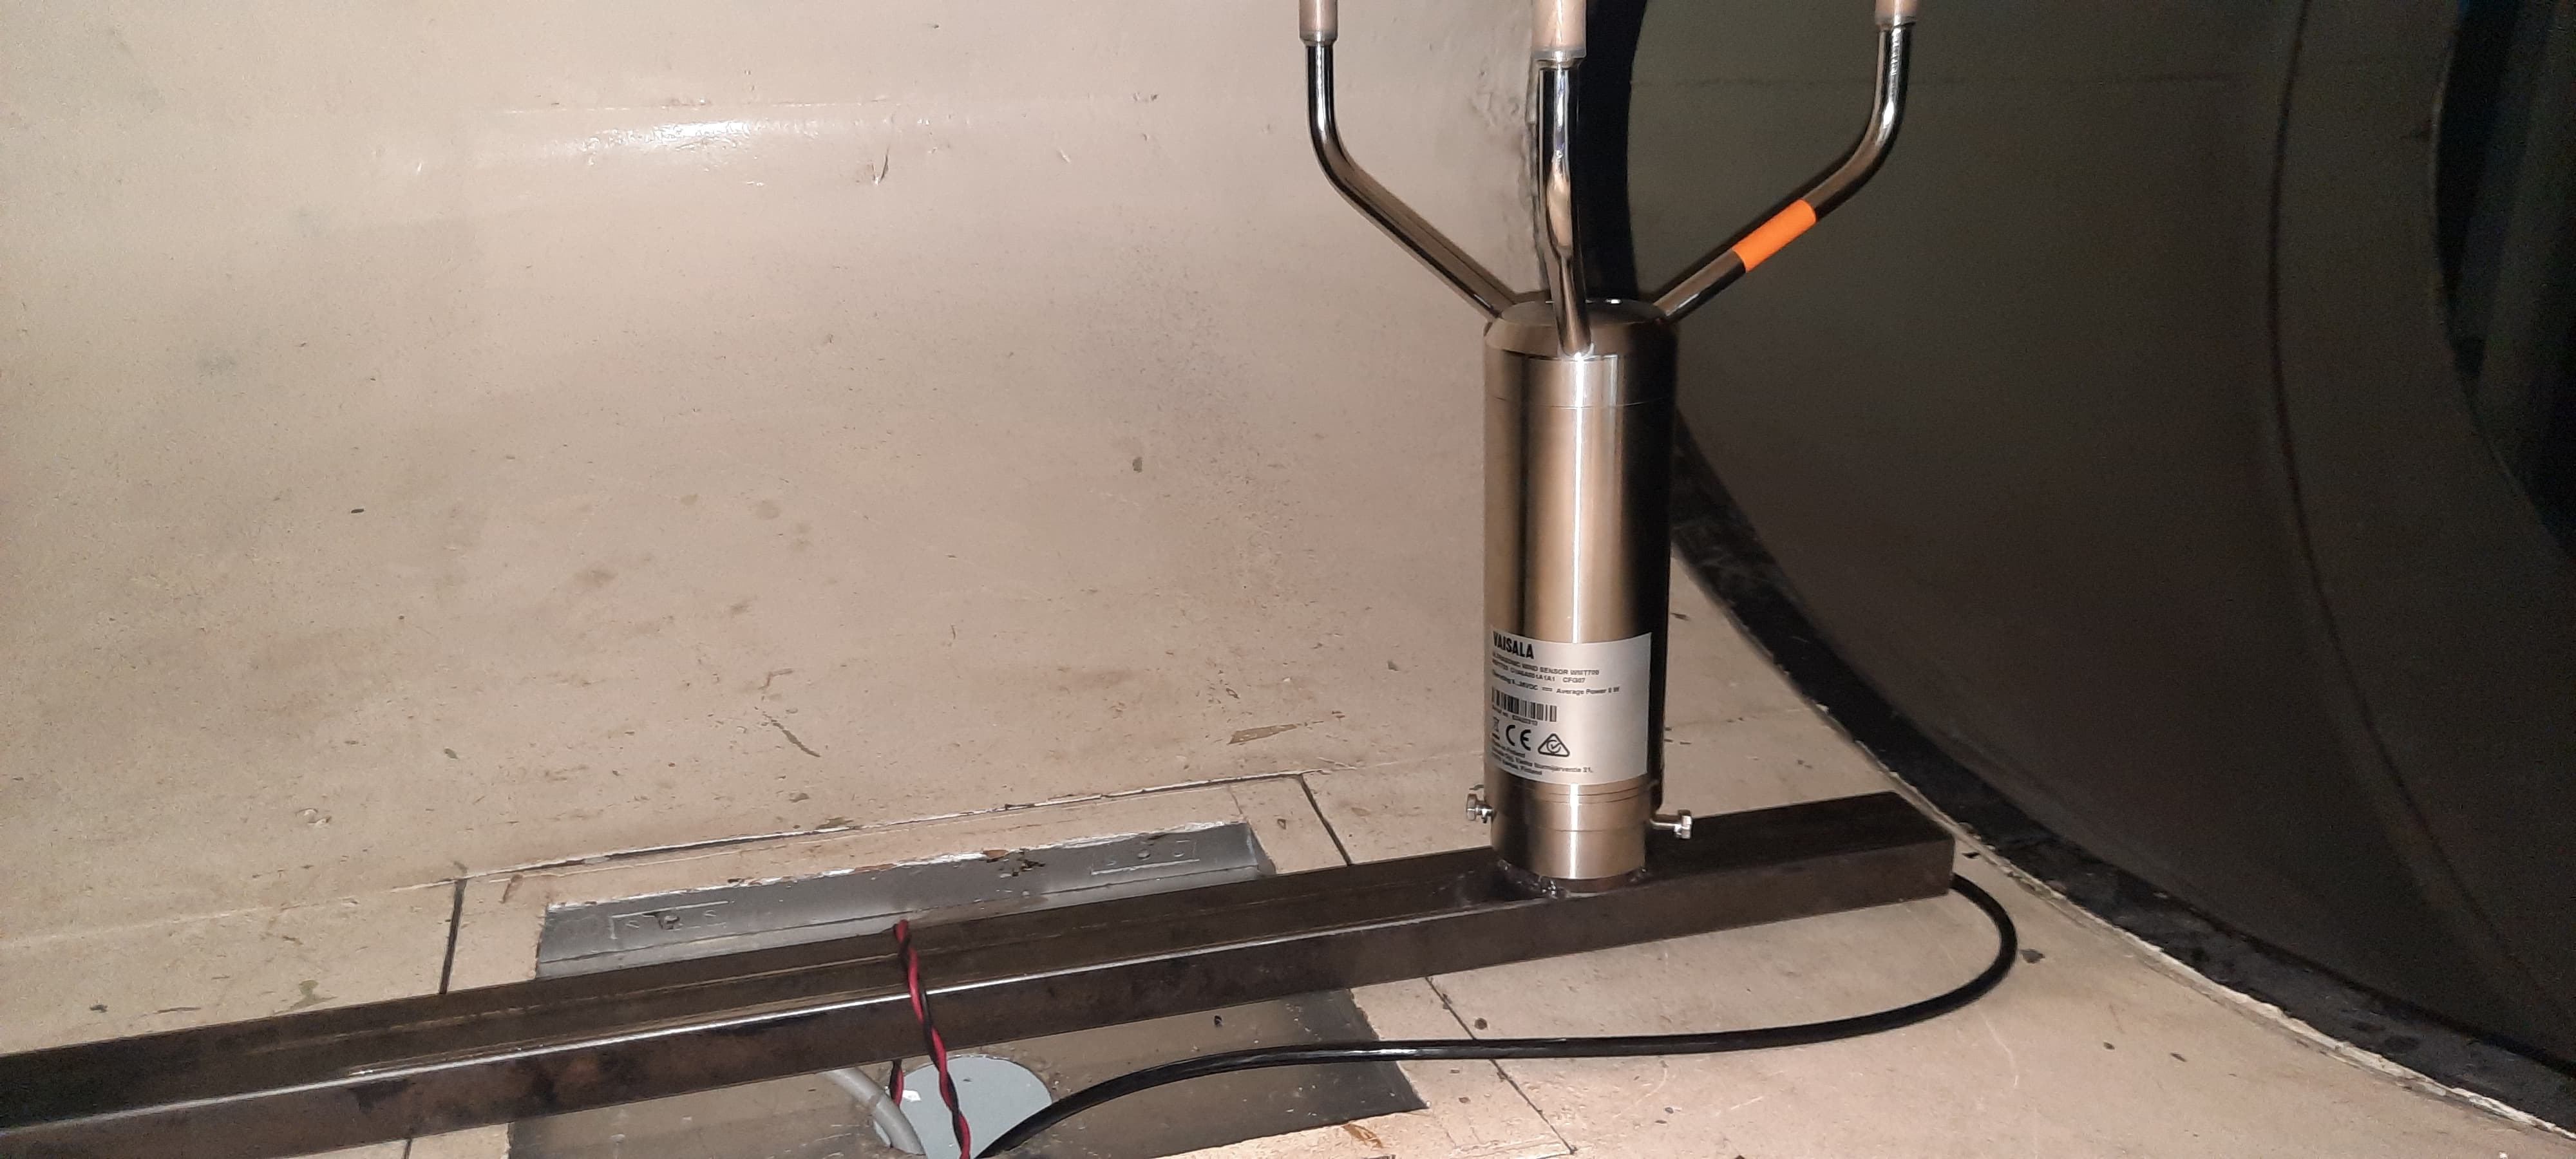
\includegraphics[width=\textwidth]{Figuras/resultados/caracterizacion/60cm.jpg}}
    \end{minipage}
    
    \caption{En (a) se muestra el anemómetro midiendo a \SI{-20}{\centi\meter}, en (b) se muestra midiendo a \SI{20}{\centi\meter} y en (c) se encuentra midiendo a \SI{60}{\centi\meter}.}
    \label{fig:caracterPuntos}
\end{figure}

En la figura \ref{fig:velocidadViento} se observan las velocidades del viento para las distintas posiciones en los cinco puntos de viento programados. El sistema de control PID se encarga de suministrar la potencia necesaria para que el viento dentro del túnel, en la posición del sensor patrón, alcance y se estabilice en el valor configurado.

\begin{figure}[H]
    \centering
    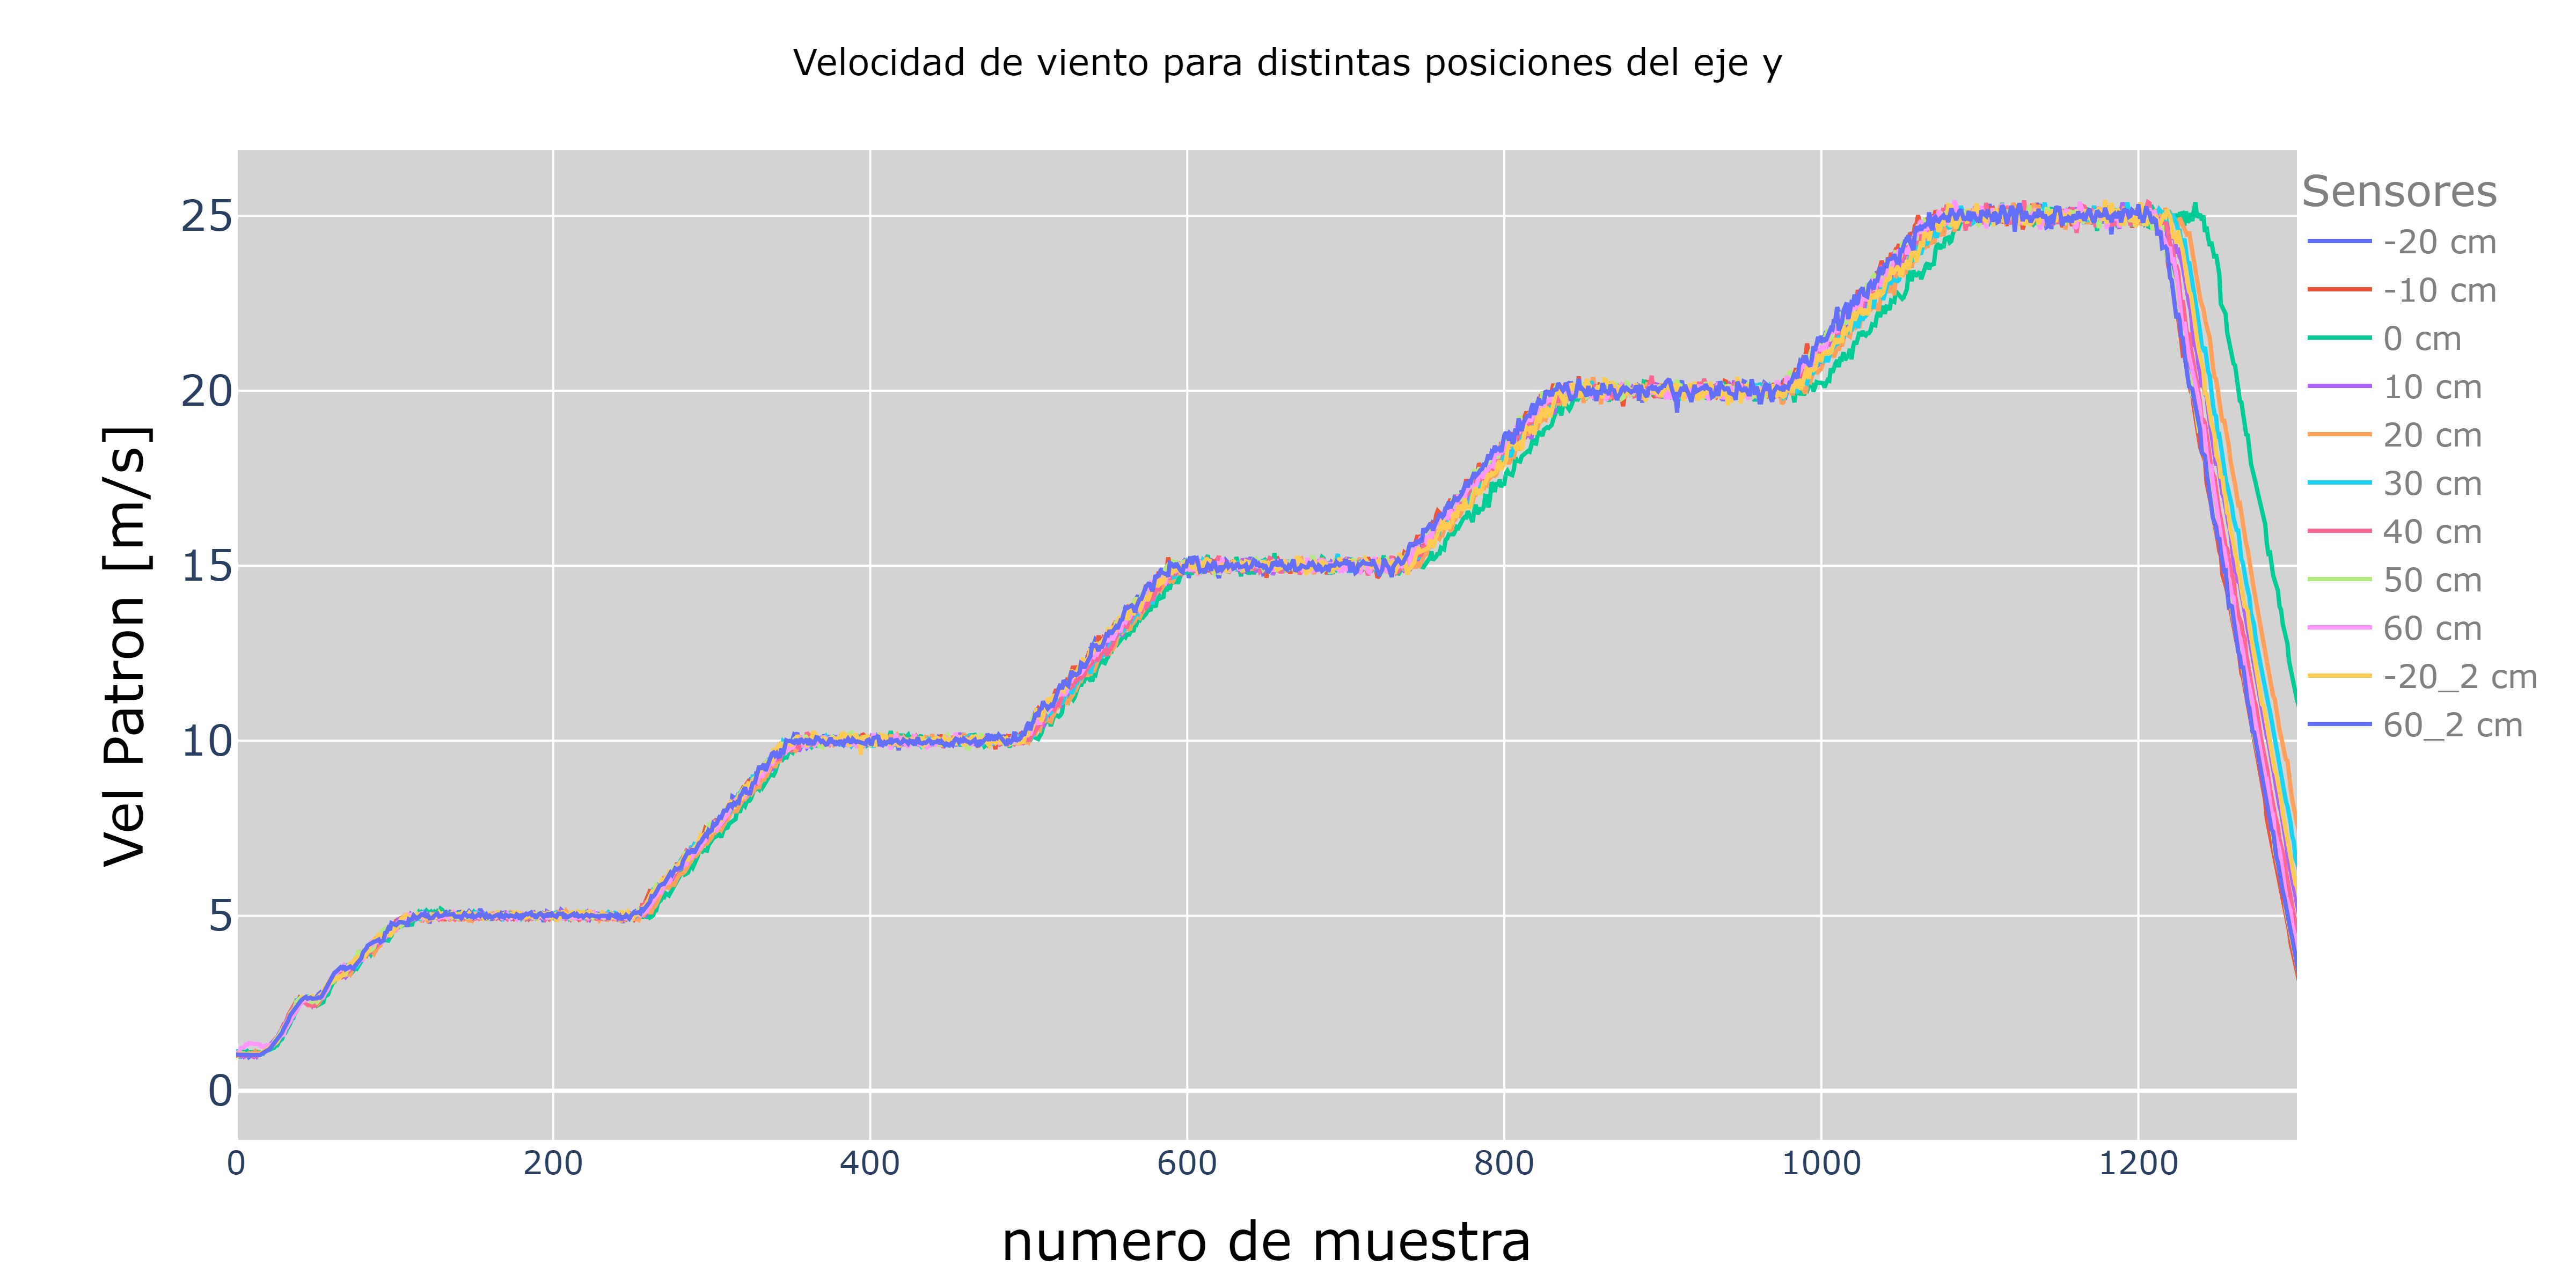
\includegraphics[width=0.95\linewidth]{Figuras/resultados/caracterizacion/velocidadViento.png}
    \caption{Velocidad de viento en cinco puntos para distintas posiciones del eje longitudinal.}
    \label{fig:velocidadViento}
\end{figure}

% Los resultados de las mediciones del nivel de modulación por ancho de pulso (PWM) para cada posición, correspondientes a las cinco velocidades configuradas, se ilustran en la Figura \ref{fig:pwmCaracterizacion}. Se puede apreciar que, para una misma velocidad de viento, pero en diferentes posiciones a lo largo del eje longitudinal, el sensor requiere distintos ciclos de trabajo que se denotan como valores enteros, entre 0 y 255, definido como el nivel de PWM, para generar la misma velocidad de viento.

El nivel de modulación por ancho de pulso (nivel de PWM) utilizado para controlar el túnel de viento es generado por el \textit{datalogger}. Este valor varía entre 0 y 255, lo que corresponde a un rango de ciclo de trabajo del 0\% al 100\%. En la Figura \ref{fig:pwmCaracterizacion} se observa  los resultados de las mediciones del nivel de PWM para cada posición del sensor patrón correspondiente a las velocidades configuradas. Se observa que, para generar un mismo valor de velocidad del viento, pero en diferentes posiciones a lo largo del eje longitudinal, el sensor requiere distinto nivel de PWM.



% para cada posición, correspondientes a las cinco velocidades configuradas, se ilustran en la Figura \ref{fig:pwmCaracterizacion}. Se observa que, para generar una misma velocidad del viento, pero en diferentes posiciones a lo largo del eje longitudinal, el sensor requiere distintos ciclos de trabajo.


\begin{figure}[H]
    \centering
    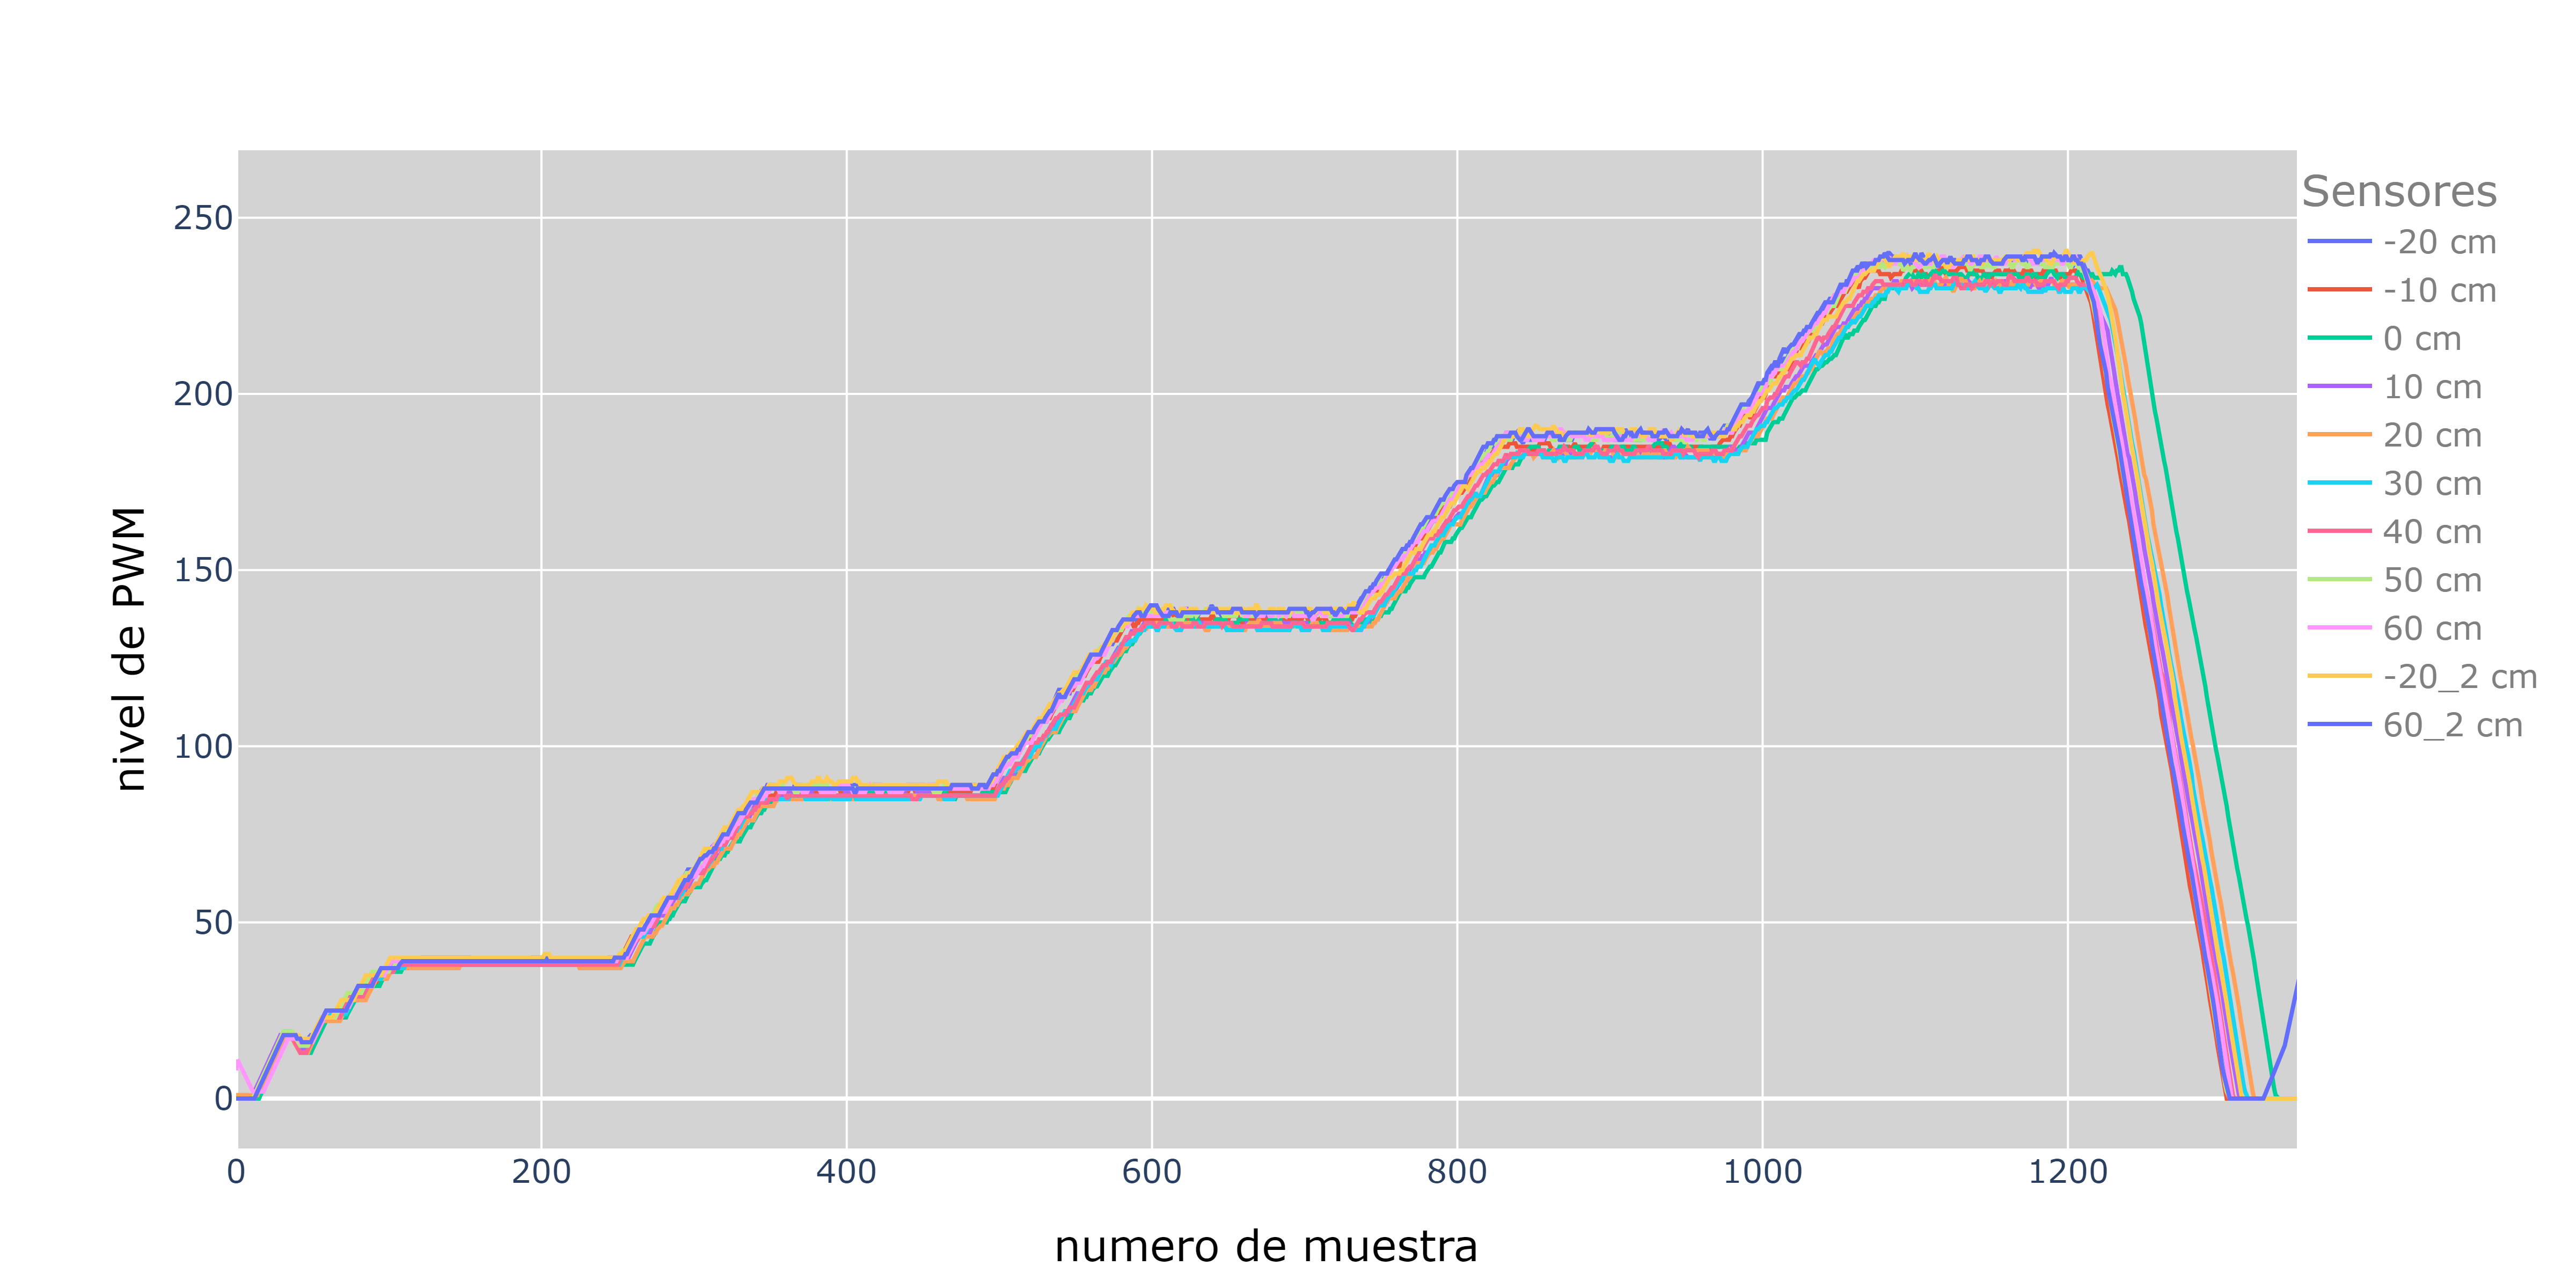
\includegraphics[width=0.95\linewidth]{Figuras/resultados/caracterizacion/pwmCaracterizacion.png}
    \caption{Nivel de PWM medido en el controlador, para distintas posiciones, obtenidas utilizando el software y hardware desarrollados en capítulos anteriores.}
    \label{fig:pwmCaracterizacion}
\end{figure}




En la Figura \ref{fig:pwmCaract25}, se realiza un acercamiento a las mediciones en \SI{25}{\meter\per\second}, donde se pueden observar las variaciones de los niveles de PWM para la misma velocidad en función de la posición. Se destaca que para posiciones entre \SI{0}{\centi\meter} y \SI{40}{\centi\meter}, los niveles de PWM son más bajos, oscilando entre 229 y 235. Sin embargo, para posiciones alejadas a izquierda y posiciones más en el centro del túnel, como \SI{-10}{\centi\meter}, \SI{-20}{\centi\meter}, \SI{50}{\centi\meter} y \SI{60}{\centi\meter}, los niveles de PWM son más altos, aunque en promedio similares entre sí. 

\begin{figure}[H]
    \centering
    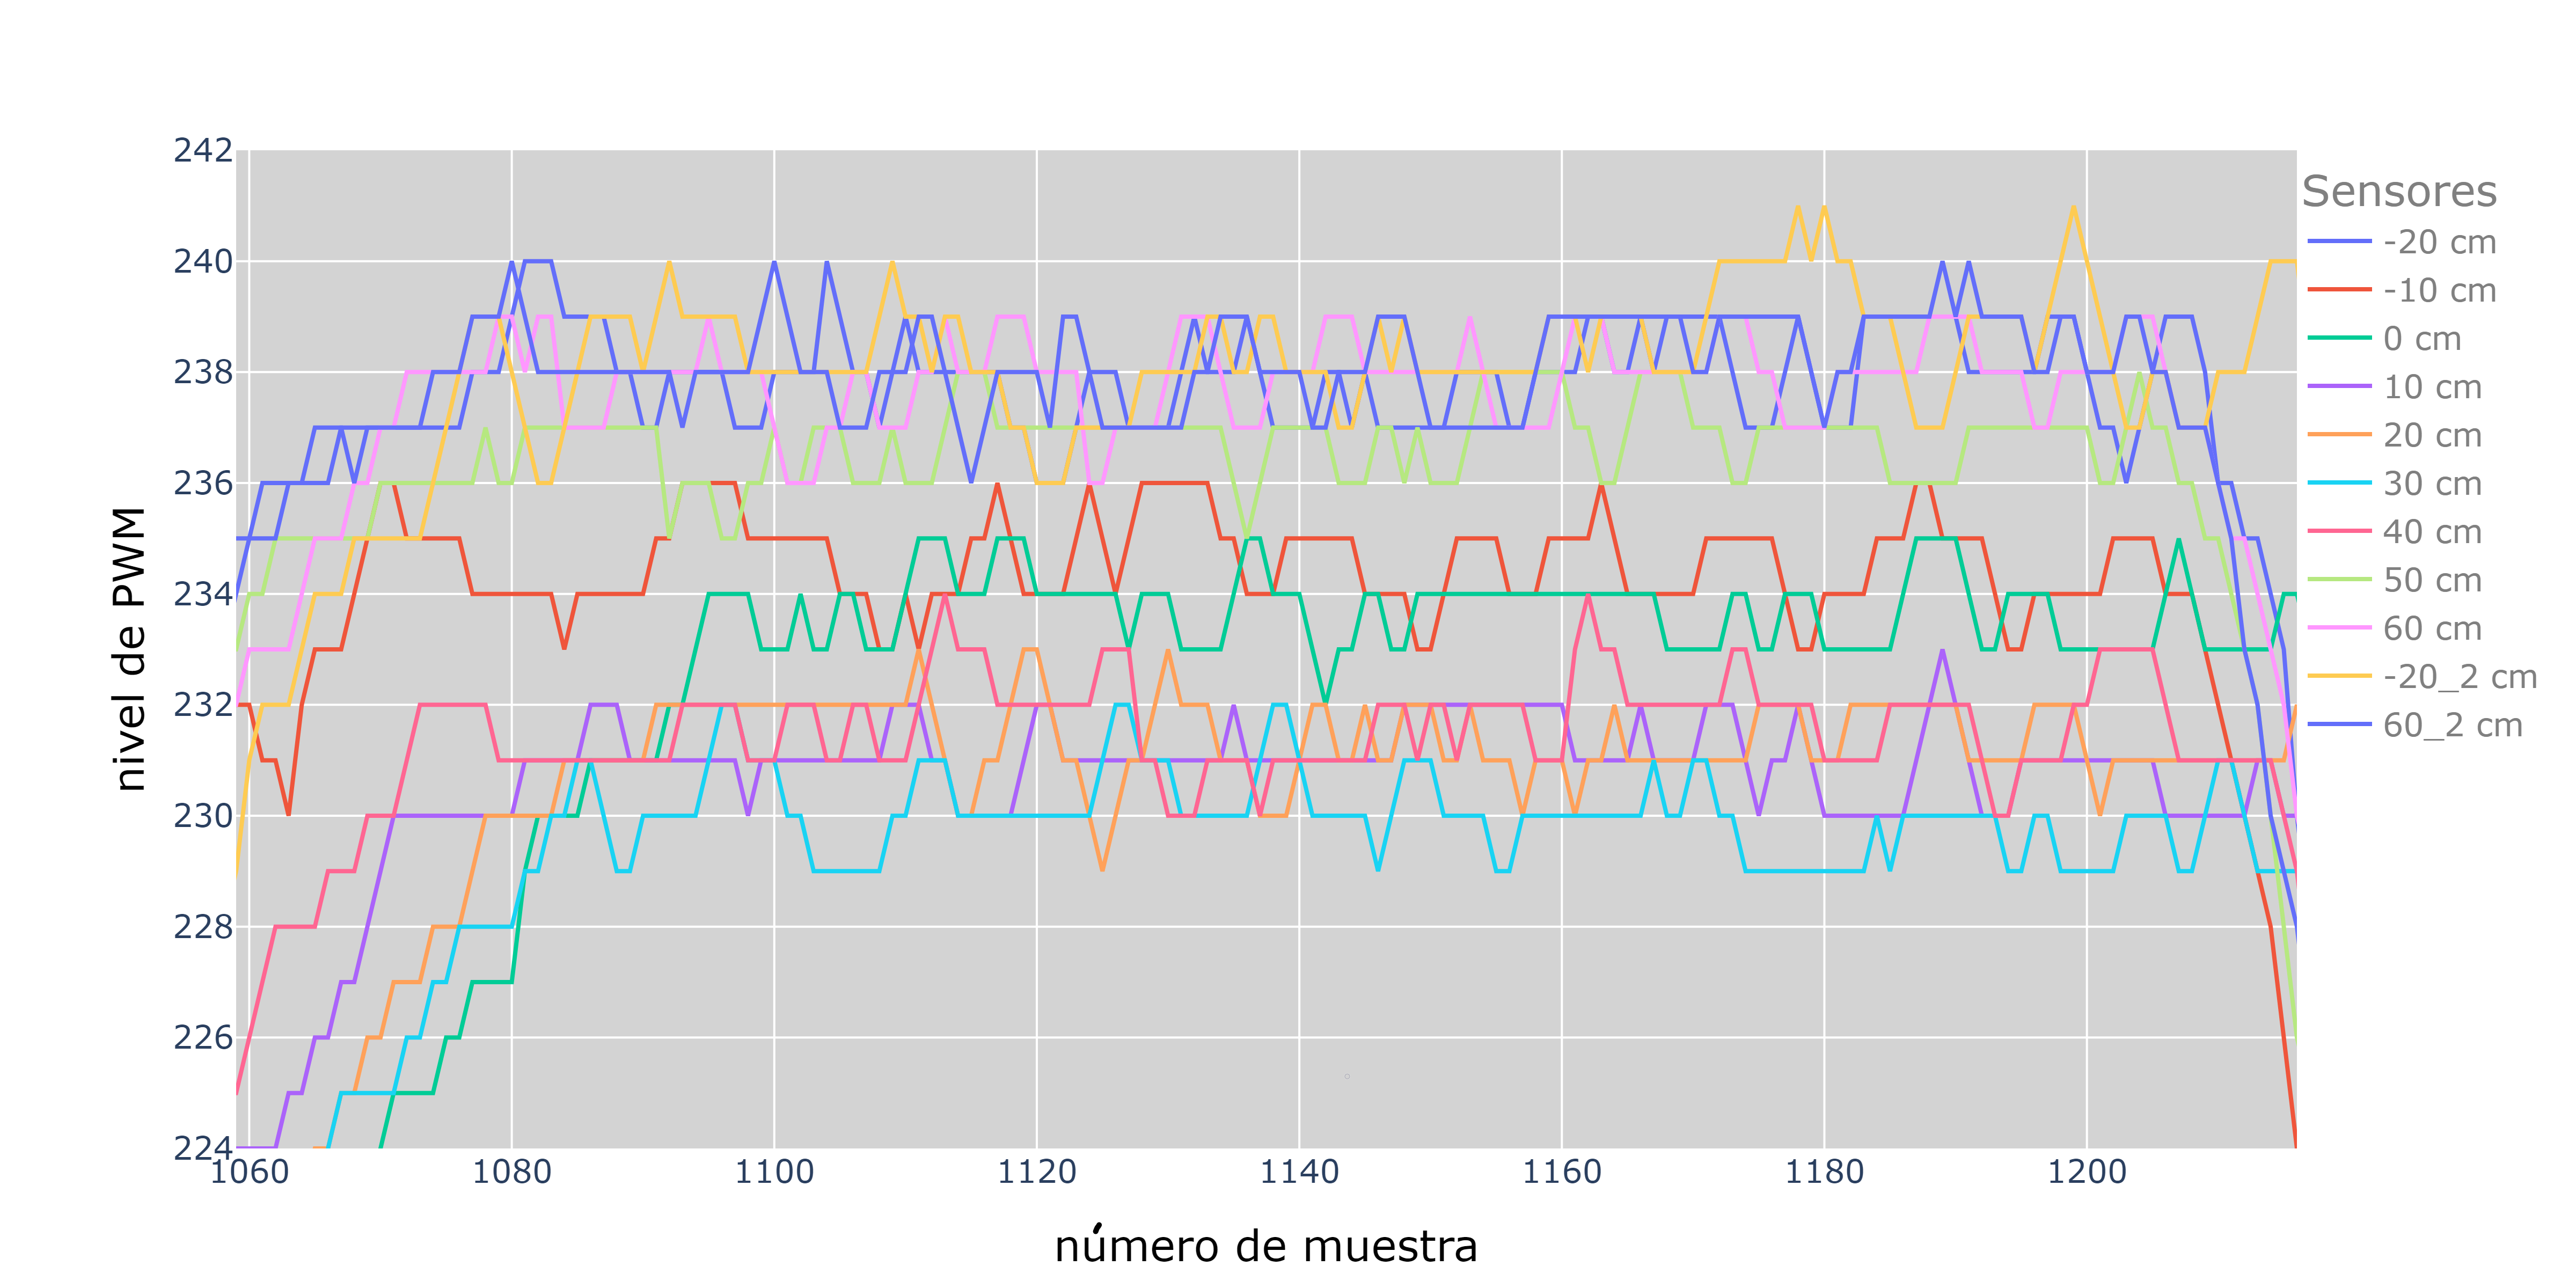
\includegraphics[width=0.95\linewidth]{Figuras/resultados/caracterizacion/pwmCaract25.png}
    \caption{Niveles de PWM para distintas posiciones del anemómetro a \SI{25}{\meter\per\second}.}
    \label{fig:pwmCaract25}
\end{figure}
% Considerando lo anterior y basándose en los resultados gráficos, se concluye que los valores de PWM necesarios para obtener una velocidad determinada son equivalentes en las posiciones de \SI{-20}{\centi\meter} y entre \SI{40}{\centi\meter} y \SI{50}{\centi\meter}. Esto asegura que los sensores estén separados entre \SI{60}{\centi\meter} y \SI{70}{\centi\meter}.
Considerando lo anterior y basándose en los resultados gráficos, se concluye que posicionando un sensor en \SI{-20}{\centi\meter} o entre \SI{40}{\centi\meter} y \SI{50}{\centi\meter} los niveles de PWM son equivalentes para obtener condiciones de flujo de aire idénticas. Además si ponemos dos sensores en esas posiciones logramos que tengan una separación de entre \SI{60}{\centi\meter} y \SI{70}{\centi\meter} lo cual es importante para minimizar el bloqueo cruzado \cite{IEC61400-12-1} \cite{ISO16622}. En la Figura \ref{fig:pwmCaractOptima}, se muestran dos curvas correspondientes a \SI{-20}{\centi\meter}, dos a \SI{60}{\centi\meter} y una a \SI{50}{\centi\meter}. Aquí se puede apreciar que para una velocidad de viento determinada, el controlador entrega en promedio el mismo nivel de PWM, lo que indica que en estos puntos, el comportamiento del flujo de aire presenta características similares.

\begin{figure}[H]
    \centering
    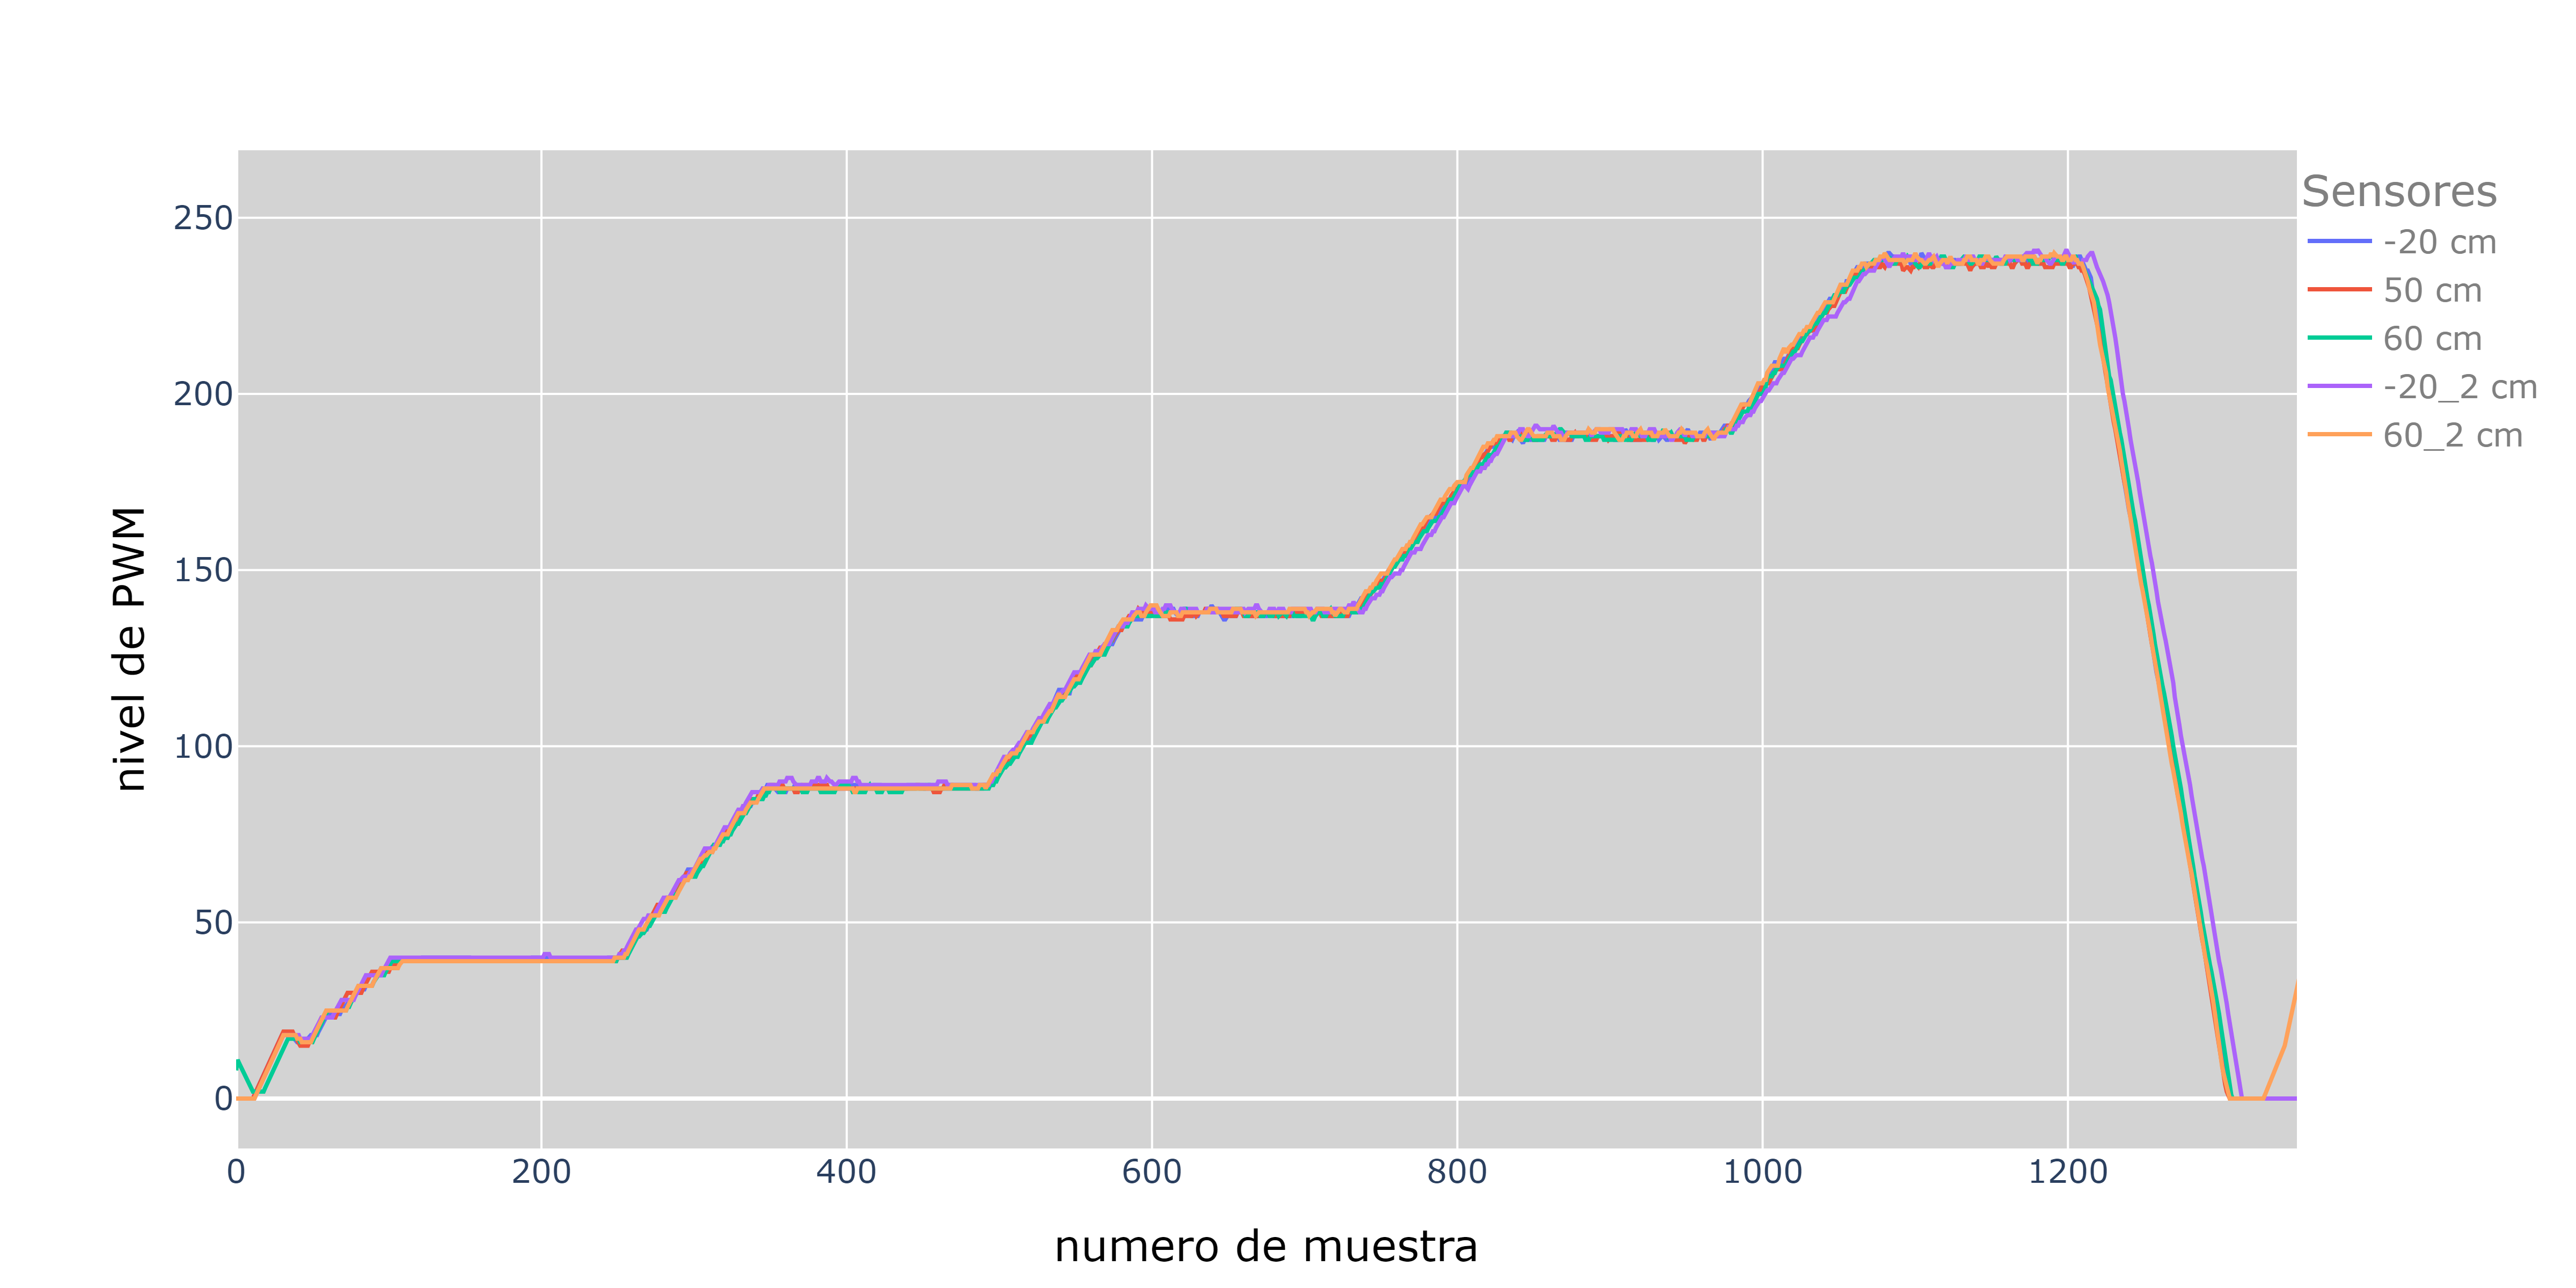
\includegraphics[width=0.95\linewidth]{Figuras/resultados/caracterizacion/pwmCaractOptima.png}
    \caption{Niveles similares de PWM para distintas posiciones del anemómetro.}
    \label{fig:pwmCaractOptima}
\end{figure}

Esta investigación proporciona una primera aproximación al comportamiento del flujo de aire dentro del túnel de viento. Sin embargo, dicha aproximación está limitada por varios factores. Por ejemplo, el sensor junto con su soporte utilizado para el análisis presenta una altura constante, lo que limita el análisis del viento en posiciones a menor altura en el eje \textit{z}. Otro problema es el área de bloqueo del sensor utilizado, donde la medición debe ser corregida. Para mejorar este tipo de ensayo, se podría utilizar un sensor con menor área de bloqueo, como un tubo Pitot o un anemómetro de hilo caliente. A pesar de estas limitaciones, como primera aproximación, es suficiente para realizar las primeras calibraciones. Esto se debe a que se garantiza que el flujo de aire en las posiciones seleccionadas tiene un comportamiento similar, generando una velocidad de viento comparable para el mismo nivel de modulación por ancho de pulso.



% \subsection{Banco de medición y configuración del hardware}
% \subsection{Configuración de la aplicación web}
% \subsection{Resultados}


% Se realizaron mediciones de 5 m/s a 25 m/s variando las distancias sobre el eje x (eje de la direccion del viento), a una altura constante en el eje z y centrado en el eje y constante, 

% \begin{itemize}
%     \item Se encontró que dos pares de puntos donde para generar una cantidad de viento se precisa aproximadamente el mismo ciclo de trabajo. Esos puntos son en -20cm y 60 cm y entre 10cm y 40 cm, 
%     \item Entre -20 y 60 cm quizá mejore el disminuya el factor de bloqueo pero en ambos casos el controlador sufre cambios mas abruptos de tensión debido a diferencia de 10 y 40 cm
%     \item Las velocidades en estos 4 puntos obtenidas a partir del controlador son relatimente estables, calcular varianza y media, de todas formas en -20 y 60 si bien estabiliza, sufre mas el controlador, con picos de tensión para mantener estable, osea le cuesta mas estabilizar en esos puntos
%     \item Entre -20 y 60 tengo una diferencia de dirección del  viento aprox de  4 grados, en cambio entre 10 y 40 tengo una diferencia en grados de 2 grados,(Para esto hacerlo bien calcular media y varianza). Ojo que esto tambien puede tener que ver en como me quedo el brazo para medir en 60, pudo haber quedado un poco inclinado y girado (repetir Medicion).
% \end{itemize}
%%%%%%%%%%%%%%%%%%%%%%%%%%%%%%%%%%%%%%%%%%%%%%%%%%%%%%%%%%%%%%%%%%%%%%%%%%%%%%%%%%%%%%%%%%%%%%%%%%%%%%%%%%%%%%%%%%%%%%%%
\section{Calibración DeltaOHM HD51.3}\label{sec:calibDeltaOhm}

Los pasos para realizar el proceso de calibración de un anemómetro se definen a continuación \cite{ISO16622} \cite{IEC61400-12-1}  \cite{procedimientoSMNLaboratorio2024}:
\begin{itemize}
    \item Ensamblar el banco de medición, montando los sensores en un soporte dentro del túnel de viento, asegurando que queden fijos y alineados correctamente.
    \item Tomar las medidas de posición de los instrumentos respecto a un sistema de referencia establecido.
    \item Medir el área de bloqueo de cada instrumento, incluyendo su soporte.
    \item Conectar los anemómetros al \textit{datalogger} y alimentar todo el sistema con una fuente de \SI{12}{V}. Además, se debe conectar el \textit{datalogger} a la red LAN local del laboratorio.
    \item Acceder a la interfaz web y configurar los parámetros de calibración, luego iniciar la adquisición de mediciones.
    \item Monitorear las mediciones mediante la interfaz web.
    \item Una vez finalizadas las mediciones, revisar si los datos obtenidos son correctos y luego activar el procesamiento y cálculo de incertidumbre.
    \item Descargar los datos y elaborar el correspondiente certificado de calibración del instrumento bajo prueba.
\end{itemize}



% \item La aplicación Django procesa las solicitudes y envía comandos al \textit{datalogger} a través de \textit{WebSocket}.
%     \item El \textit{datalogger} controla el variador de velocidad del motor mediante señales PWM, ajustando el flujo de aire en el túnel de viento.
%     \item Los datos de los anemómetros y otros sensores se registran y envían a la aplicación Django.
En base a los pasos descritos, se realizó la calibración de un sensor ultrasónico de viento marca DeltaOhm, modelo HD51.3, mostrado en la figura \ref{fig:sensorDeltaOhm}, utilizando como sensor patrón el de la figura \ref{fig:sensorVaisala}, modelo WMT700 de la marca Vaisala.

\subsection{Banco de medición y configuración del hardware}\label{sec:bancoMedicionDeltaOhm}
En la Figura \ref{fig:deltaVistaFrontal} se muestra el montaje de los sensores sobre una barra de acero, donde se instalaron con una distancia $d$ de \SI{65}{\centi\meter} y a una altura $h$ respecto a la base del soporte de \SI{36.5}{\centi\meter}. Los sensores quedan alineados y nivelados en el eje longitudinal de la barra, como se muestra en las Figuras \ref{fig:deltaVistaSup2} y \ref{fig:deltaVistaPerfil}.

\begin{figure}[H]
    \centering
    \begin{minipage}[b]{0.5\textwidth}
        % \centering
        \subcaptionbox{\label{fig:deltaVistaFrontal}}{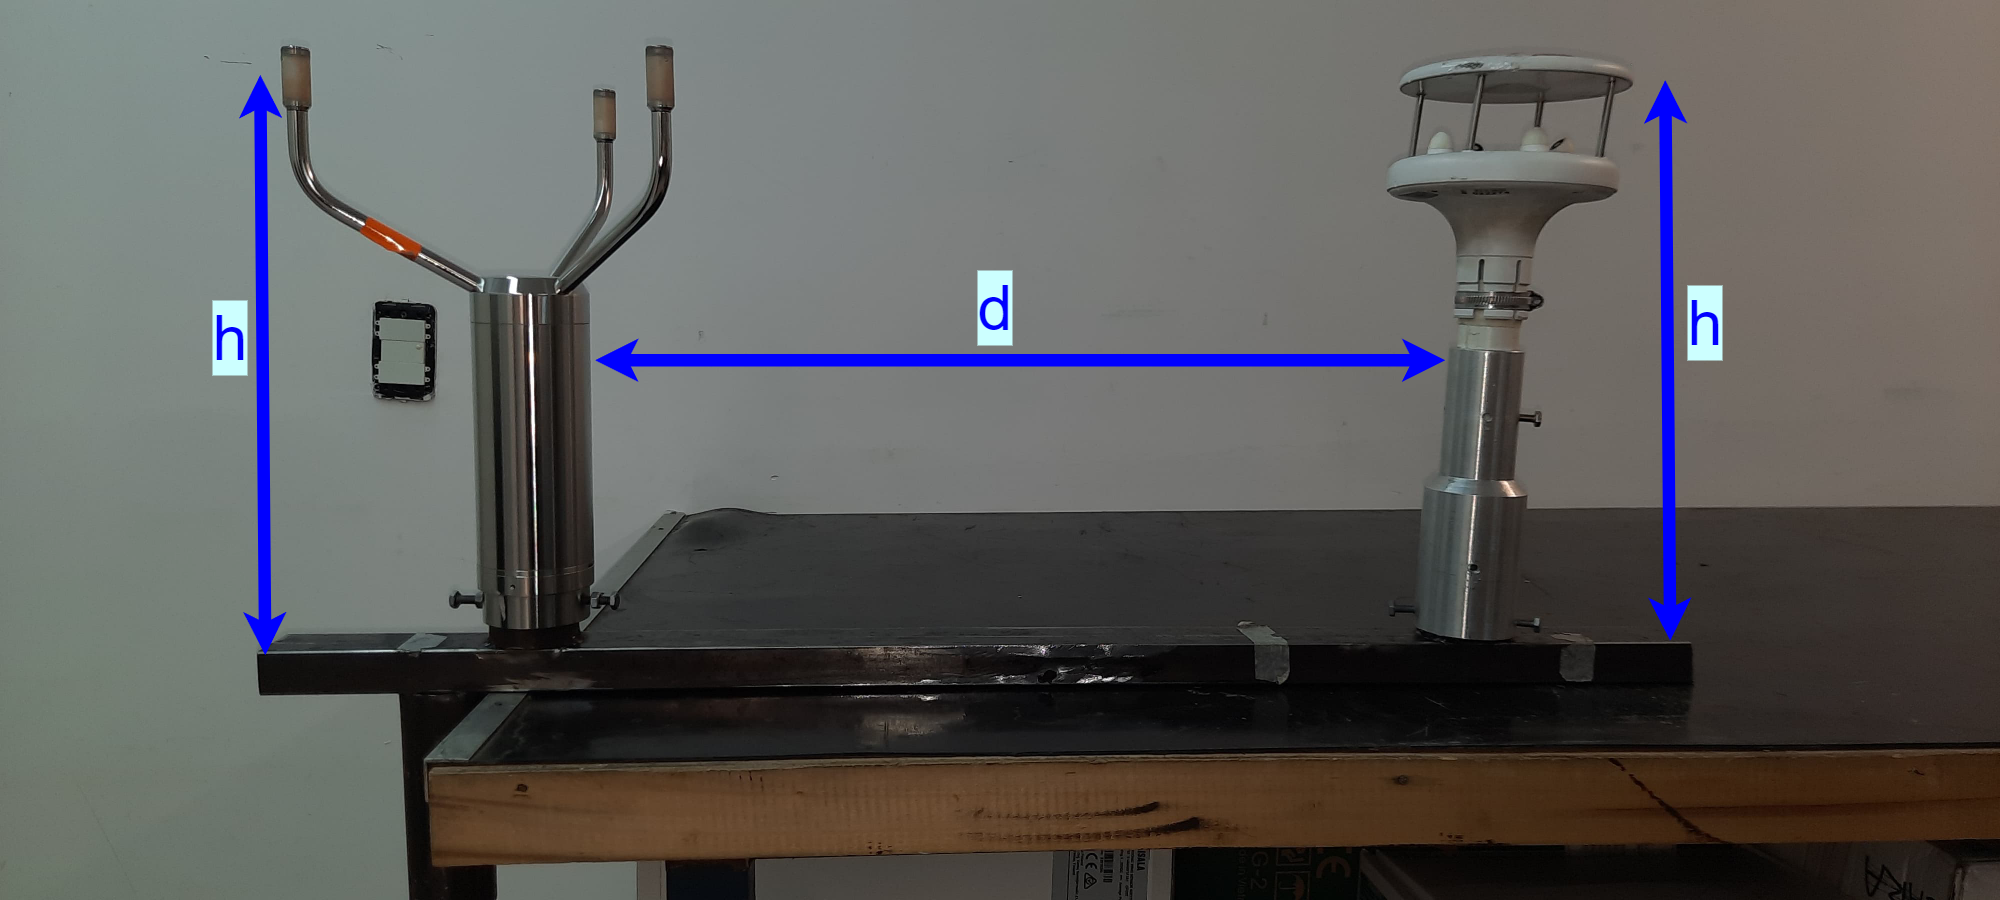
\includegraphics[width=\textwidth]{Figuras/resultados/calibracion/HD51_3/deltaVistaFrontal.png}}
        \subcaptionbox{\label{fig:deltaVistaSup2}}{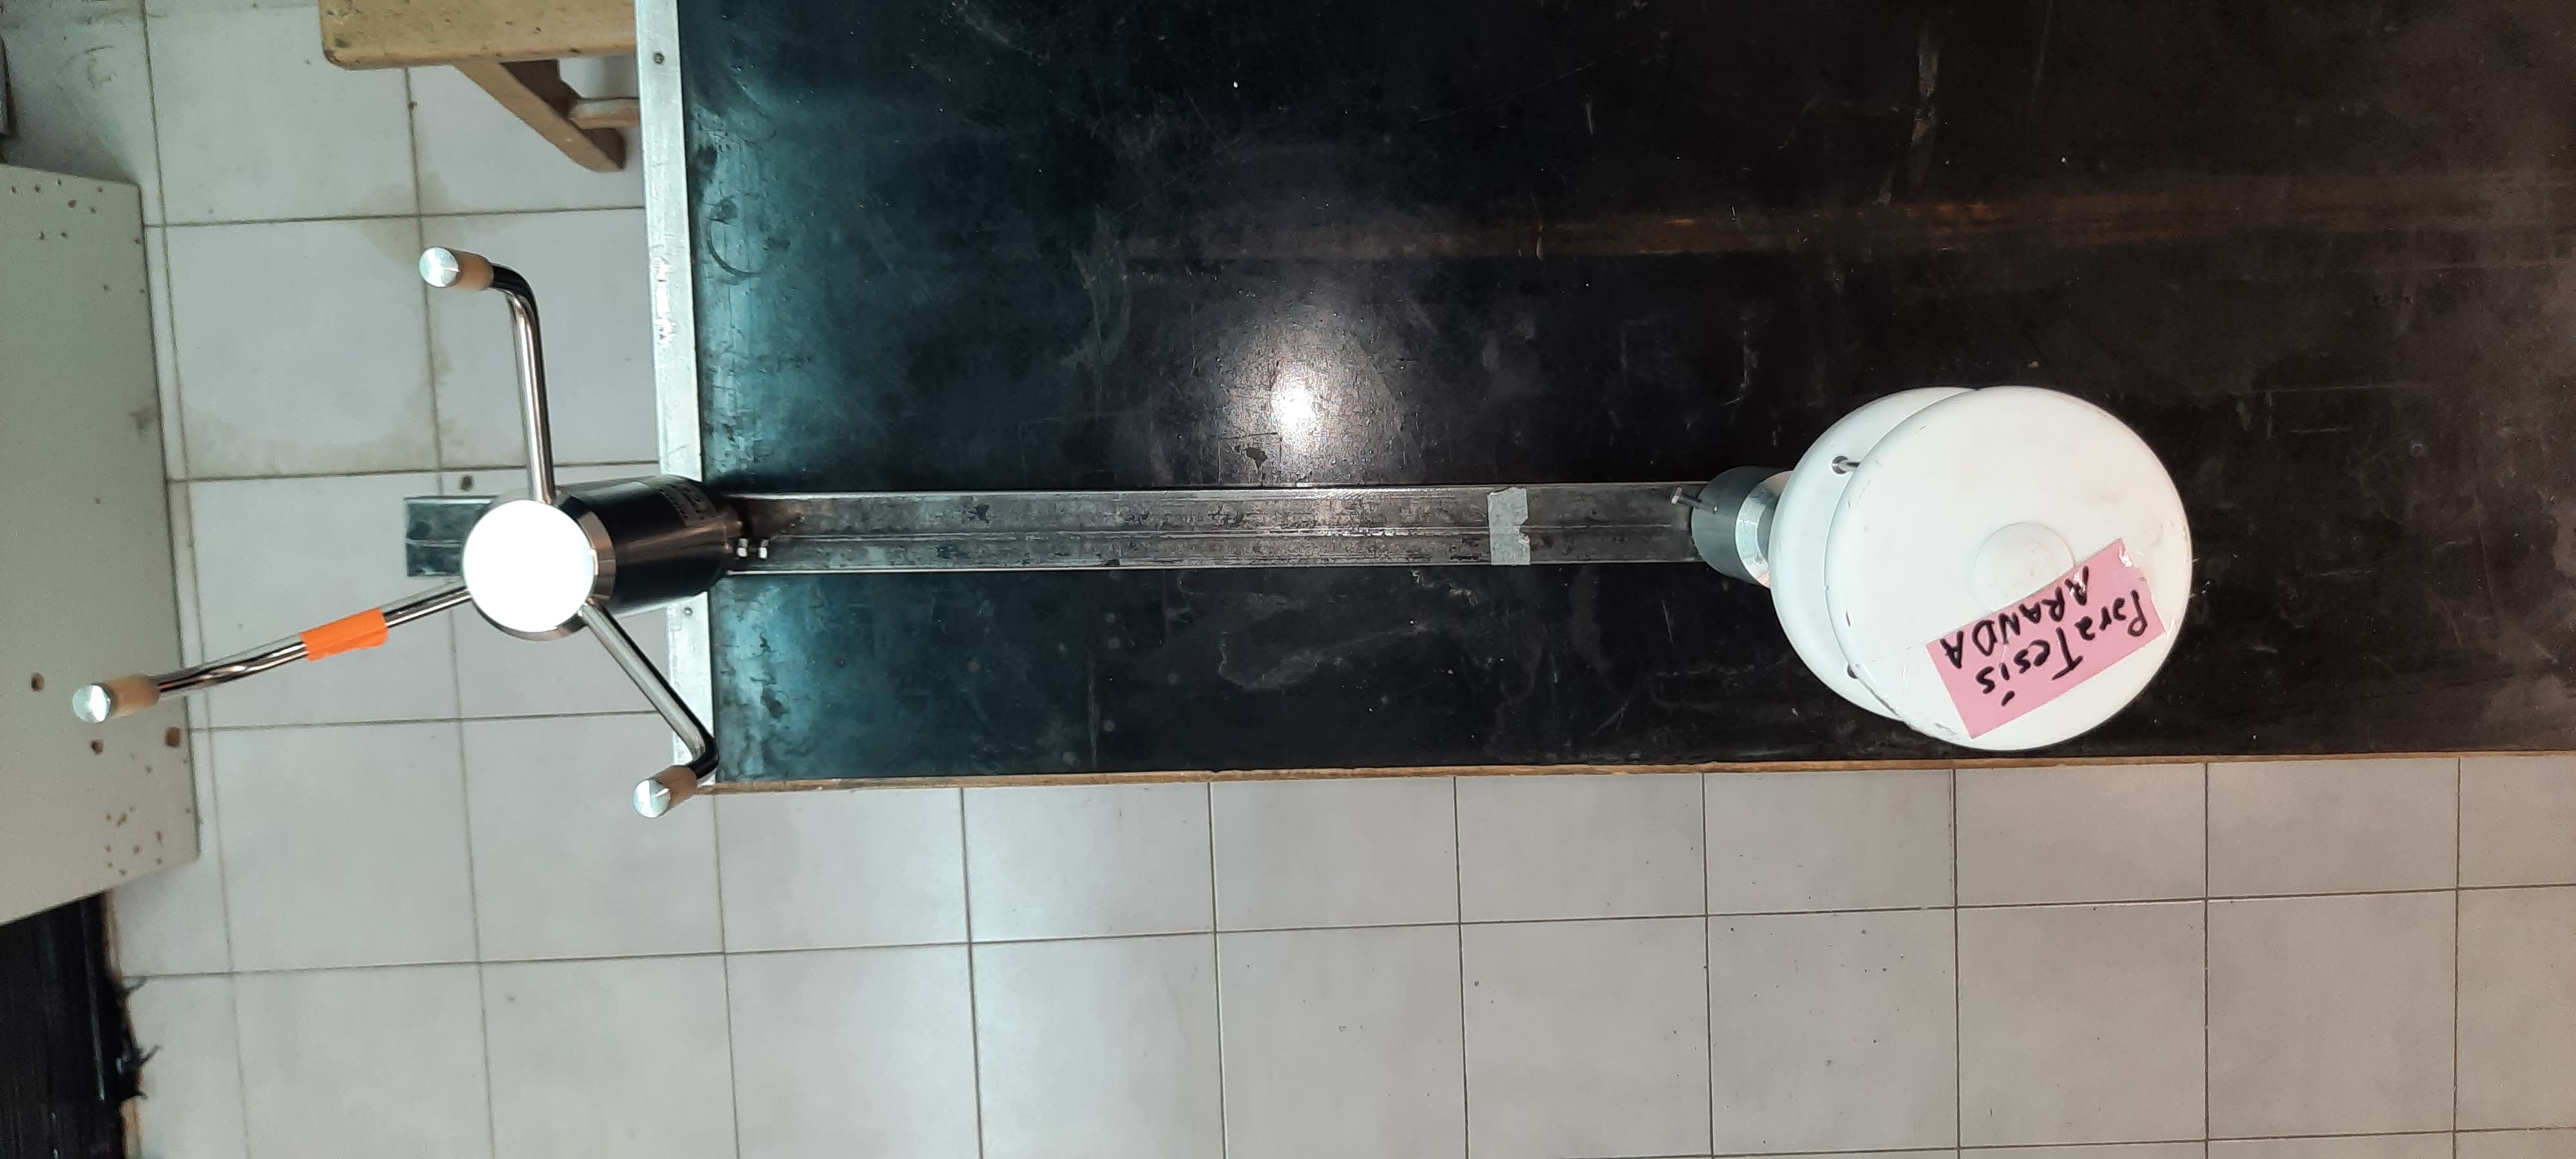
\includegraphics[width=\textwidth]{Figuras/resultados/calibracion/HD51_3/deltaVistaSup2.jpg}}
    \end{minipage}  
    \hspace{1em} % Espacio vertical entre las filas
    \begin{minipage}[b]{0.22\textwidth}
        % \centering
        \subcaptionbox{\label{fig:deltaVistaPerfil}}{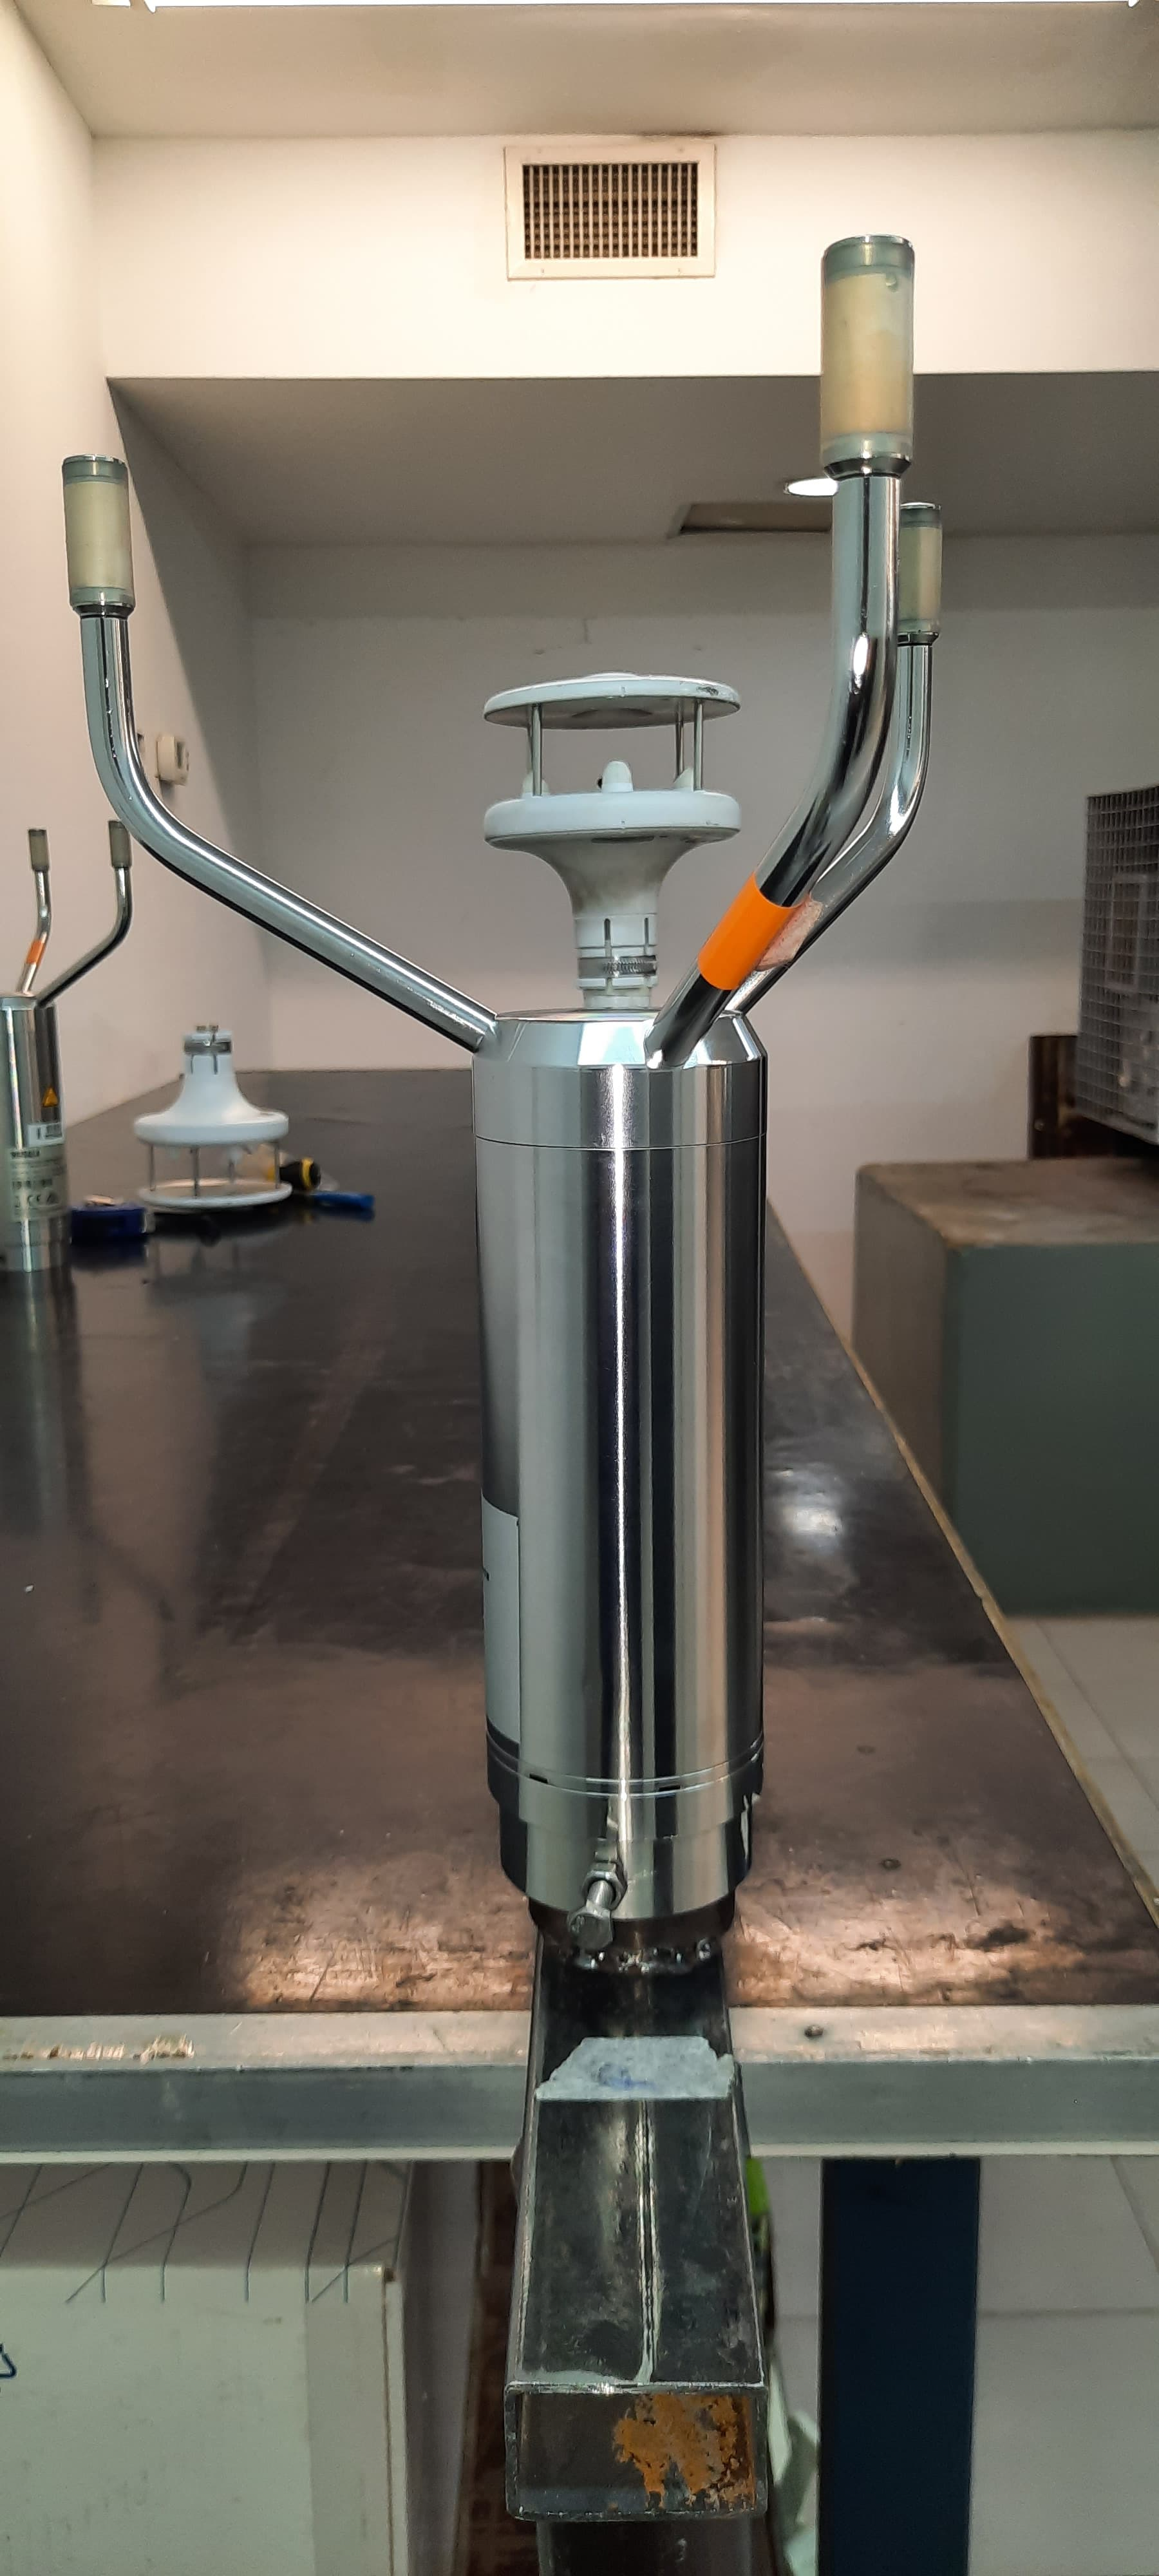
\includegraphics[width=\textwidth]{Figuras/resultados/calibracion/HD51_3/deltaVistaPerfil.jpg}}
    \end{minipage}
    \caption{En (a) se muestra la vista frontal de los sensores patrón y bajo prueba, en (b) se observa una vista superior para ver la alineación, y en (c) se muestra una vista lateral.}
    \label{fig:bancoMedicionDeltaOhm}
\end{figure} 
 
Luego de ensamblar y alinear los sensores, se debe instalar el brazo dentro del túnel de viento. Es crucial conectar previamente los cables de los sensores antes de ajustar los prisioneros. En la Figura \ref{fig:deltaMontajeTunel} se observa el sensor montado en el túnel de viento. El sensor bajo calibración se encuentra a \SI{-20}{\centi\meter} y el sensor de referencia está a \SI{45}{\centi\meter}, ambos a una altura de \SI{39.5}{\centi\meter} respecto al piso del túnel. Todo el conjunto está asegurado con la barra telescópica mostrada en la Figura \ref{fig:soporteParaBrazoConAnemos}.


\begin{figure}[H]
    \centering
    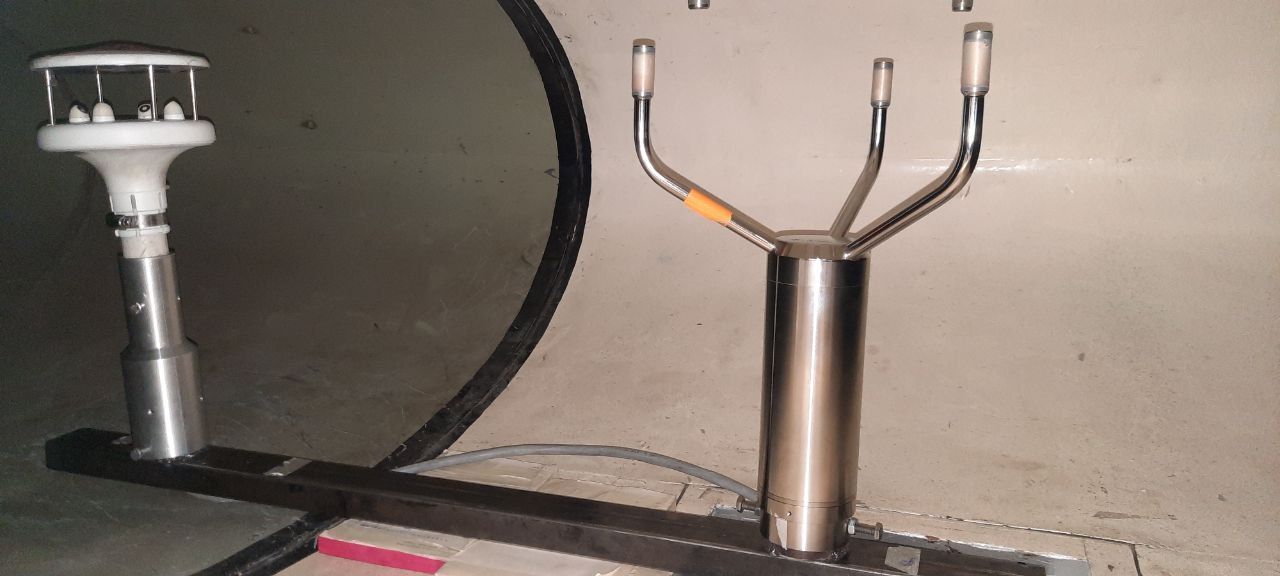
\includegraphics[width=0.7\linewidth]{Figuras/resultados/calibracion/HD51_3/deltaMontajeTunel.jpg}
    \caption{Brazo con los sensores bajo calibración a izquierda y patrón a derecha dentro del túnel.}
    \label{fig:deltaMontajeTunel}
\end{figure}

Como se observa en la Figura \ref{fig:datalogger3}, en la mesa de trabajo se instala el datalogger, al cual se conectan el sensor bajo calibración y el sensor patrón a través de sus puertos RS485. Tanto los sensores como el datalogger se alimentan con una fuente de \SI{12}{\volt}. El módulo Ethernet se conecta al switch, y el nivel de tensión continua generado por el PWM se conecta al variador de velocidad del túnel.
(mejorar esta foto)
\begin{figure}[H]
    \centering
    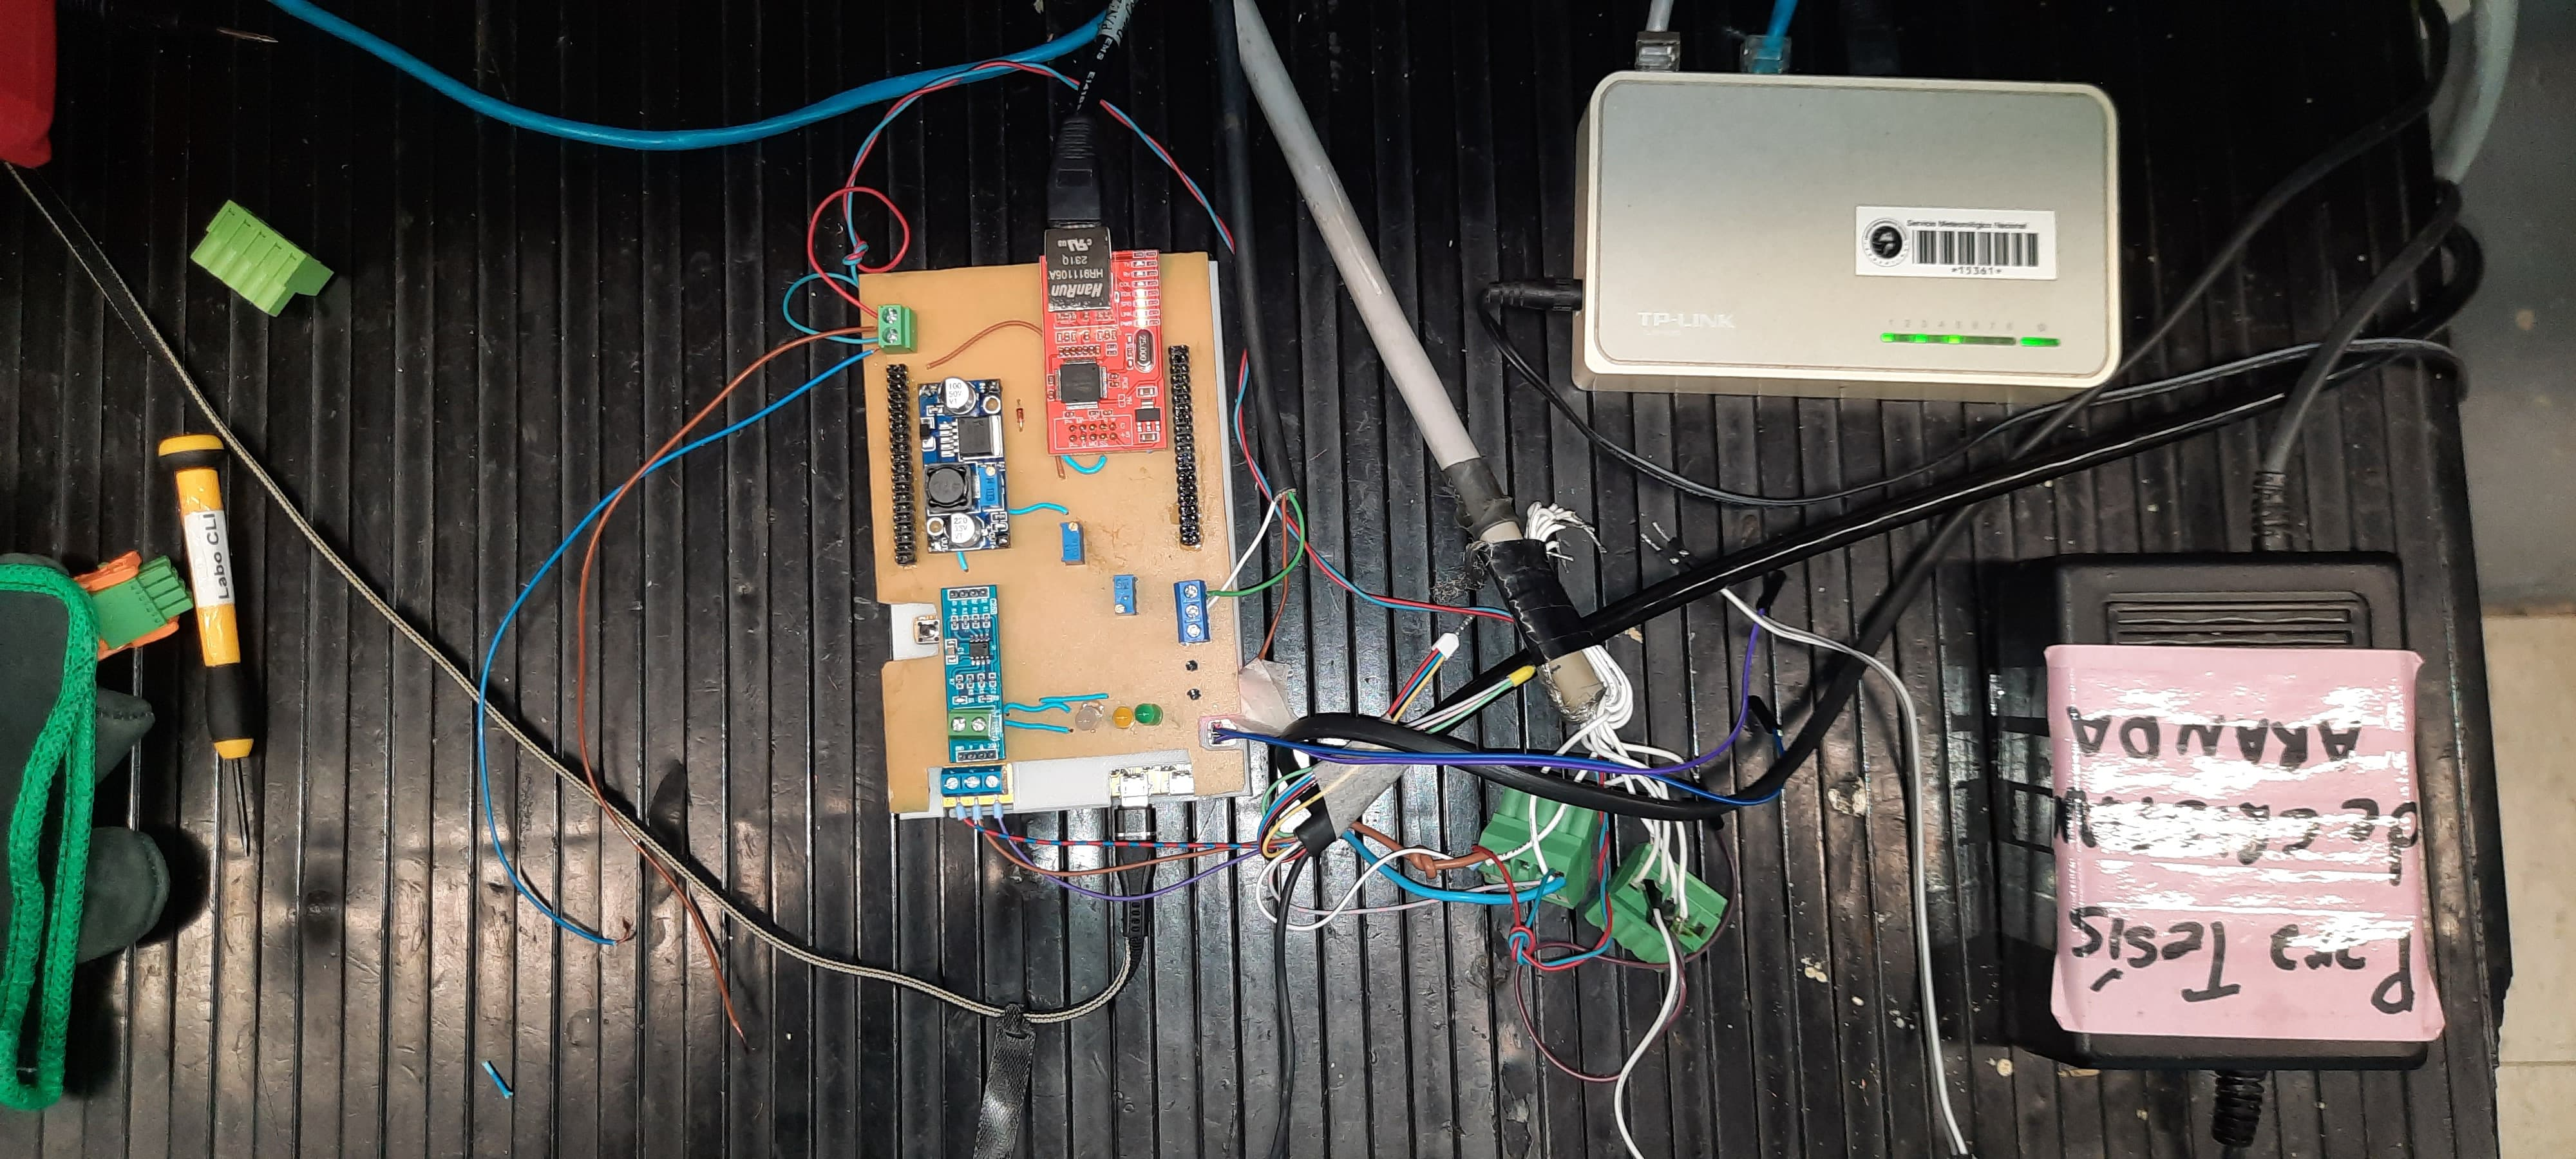
\includegraphics[width=0.7\linewidth]{Figuras/resultados/calibracion/datalogger3.jpg}
    \caption{Mesa de trabajo con el datalogger y los insumos necesarios para su funcionamiento.}
    \label{fig:datalogger3}
\end{figure}

\subsection{Configuración de la aplicación web}

En las Figuras \ref{fig:configSensorIBC} y \ref{fig:configSensorPAT} se muestra la carga de metadatos de los sensores. En la Figura \ref{fig:configCertiCalibracion} se presenta la carga de datos del certificado de calibración del sensor patrón. Por otro lado, en la Figura \ref{fig:configCertiCaracTunel} se muestra los datos de certificado de caracterización del túnel de viento, los valores se cargan como nulos, ya que aún no se ha realizado el estudio de homogeneidad y estabilidad de la zona de medición. Estos valores nulos aportan una incertidumbre nula al presupuesto de incertidumbre. No obstante, una vez realizados estos estudios, se podrán agregar los valores obtenidos sin mayor dificultad, y el sistema incorporará su aporte de incertidumbre al presupuesto.


\begin{figure}[H]
    \centering
    \begin{minipage}[b]{0.2\textwidth}
        \centering
        \subcaptionbox{\label{fig:configSensorIBC}}{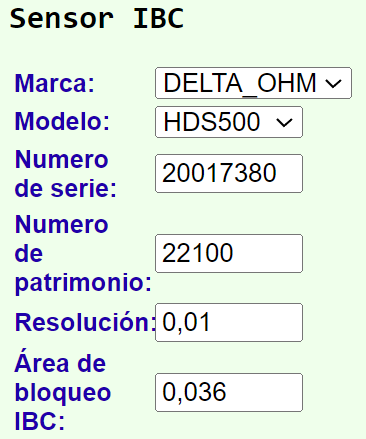
\includegraphics[width=\textwidth]{Figuras/resultados/calibracion/HD51_3/configSensorIBC.png}}
    \end{minipage}  
    \hspace{0.5em} % Espacio vertical entre las filas
    \begin{minipage}[b]{0.18\textwidth}
        \centering
        \subcaptionbox{\label{fig:configSensorPAT}}{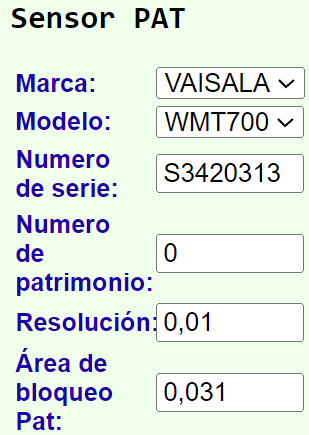
\includegraphics[width=\textwidth]{Figuras/resultados/calibracion/HD51_3/configSensorPAT.png}}
    \end{minipage}
    \hspace{1em} % Espacio vertical entre las filas
    \begin{minipage}[b]{0.23\textwidth}
        \centering
        \subcaptionbox{\label{fig:configCertiCalibracion}}{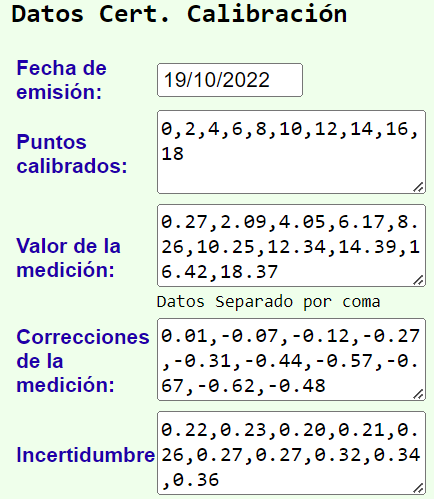
\includegraphics[width=\textwidth]{Figuras/resultados/calibracion/HD51_3/configCertiCalibracion.png}}
    \end{minipage}  
    \hspace{0.5em} % Espacio vertical entre las filas
    \begin{minipage}[b]{0.28\textwidth}
        \centering
        \subcaptionbox{\label{fig:configCertiCaracTunel}}{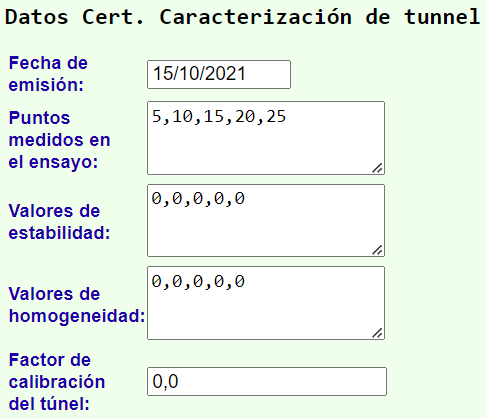
\includegraphics[width=\textwidth]{Figuras/resultados/calibracion/HD51_3/configCertiCaracTunel.png}}
    \end{minipage}  
    \caption{En (a), (b), (c) y (d) se muestran los metadatos ingresados el por el usuario para realizar la calibración.}
    \label{fig:configMetadatos}
\end{figure} 

En la figura \ref{fig:configDataloggerDelta} se muestra la configuración del datalogger. Se elige un tiempo de muestreo de \SI{1}{\second} y un tiempo de tabla también de \SI{1}{\second}, ya que nos interesa el dato instantáneo para realizar la calibración. Se selecciona el puerto COM2 (RS485 agregado con el módulo RS485-TTL) para el IBC y el puerto COM1 (RS485 propio de la EDU-CIAA) para el sensor patrón. Ambos sensores tienen un baud rate de \SI{9600}{}. En la Figura \ref{fig:configTunelDelta} se muestra la configuración del túnel de viento. Se establece un punto mínimo de \SI{1}{\meter\per\second} y un punto máximo de \SI{25}{\meter\per\second}. Se indican 5 puntos para calibrar en \SI{5}{\meter\per\second}, \SI{10}{\meter\per\second}, \SI{15}{\meter\per\second}, \SI{20}{\meter\per\second} y \SI{25}{\meter\per\second}. Se configura un ciclo ascendente-descendente de \SI{5}{\meter\per\second} a \SI{25}{\meter\per\second} y luego de \SI{25}{\meter\per\second} a \SI{5}{\meter\per\second}. Se establece un tiempo de transición para llegar de un punto a otro de \SI{3}{\minute}, un tiempo para estabilizar las mediciones de \SI{5}{\minute} y un tiempo de medición de \SI{2}{\minute}.

\begin{figure}[H]
    \centering
    \begin{minipage}[b]{0.18\textwidth}
        \centering
        \subcaptionbox{\label{fig:configDataloggerDelta}}{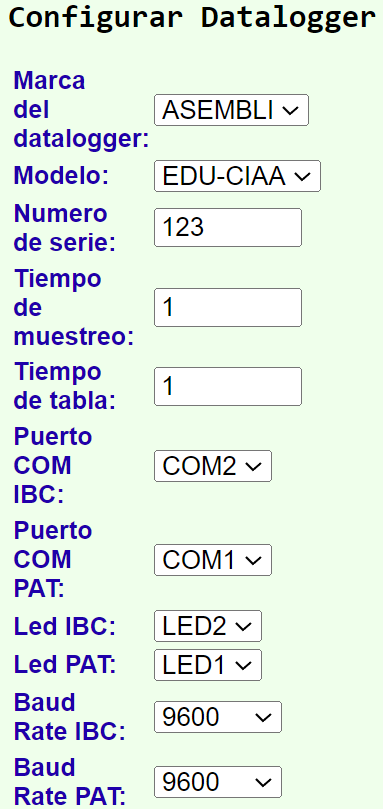
\includegraphics[width=\textwidth]{Figuras/resultados/calibracion/HD51_3/configDatalogger.png}}
    \end{minipage}  
    \hspace{1em} % Espacio vertical entre las filas
    \begin{minipage}[b]{0.23\textwidth}
        \centering
        \subcaptionbox{\label{fig:configTunelDelta}}{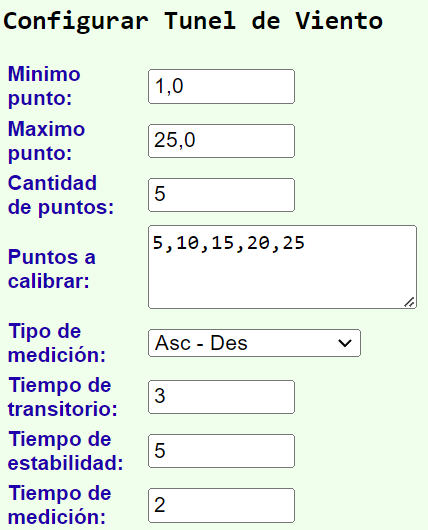
\includegraphics[width=\textwidth]{Figuras/resultados/calibracion/HD51_3/configTunel.png}}
    \end{minipage}  
    \caption{En (a) y (b) se muestra las configuraciones realizada por el operador para el datalogger y el túnel de viento.}
    \label{fig:configEquiposDelta}
\end{figure} 


\subsection{Resultados}

Una vez finalizada la adquisición de datos, se observan en las Figuras \ref{fig:deltaVelocidadCrudo} y \ref{fig:deltaDireccionCrudo} los datos crudos de intensidad y dirección del viento, respectivamente. De estos datos se extrae la parte plana de cada punto, correspondiente al tiempo de medición. En este caso, se toman muestras cada 1 segundo, y el tiempo de medición es de 2 minutos, equivalente a 120 segundos. Por lo tanto, se tienen 120 muestras por punto de viento configurado. Estas muestras se presentan en tablas, donde el operador debe verificar que en cada punto, las mediciones no se salgan del rango establecido.

\begin{figure}[H]
    \centering
    \begin{minipage}[b]{1\textwidth}
        \centering
        \subcaptionbox{\label{fig:deltaVelocidadCrudo}}{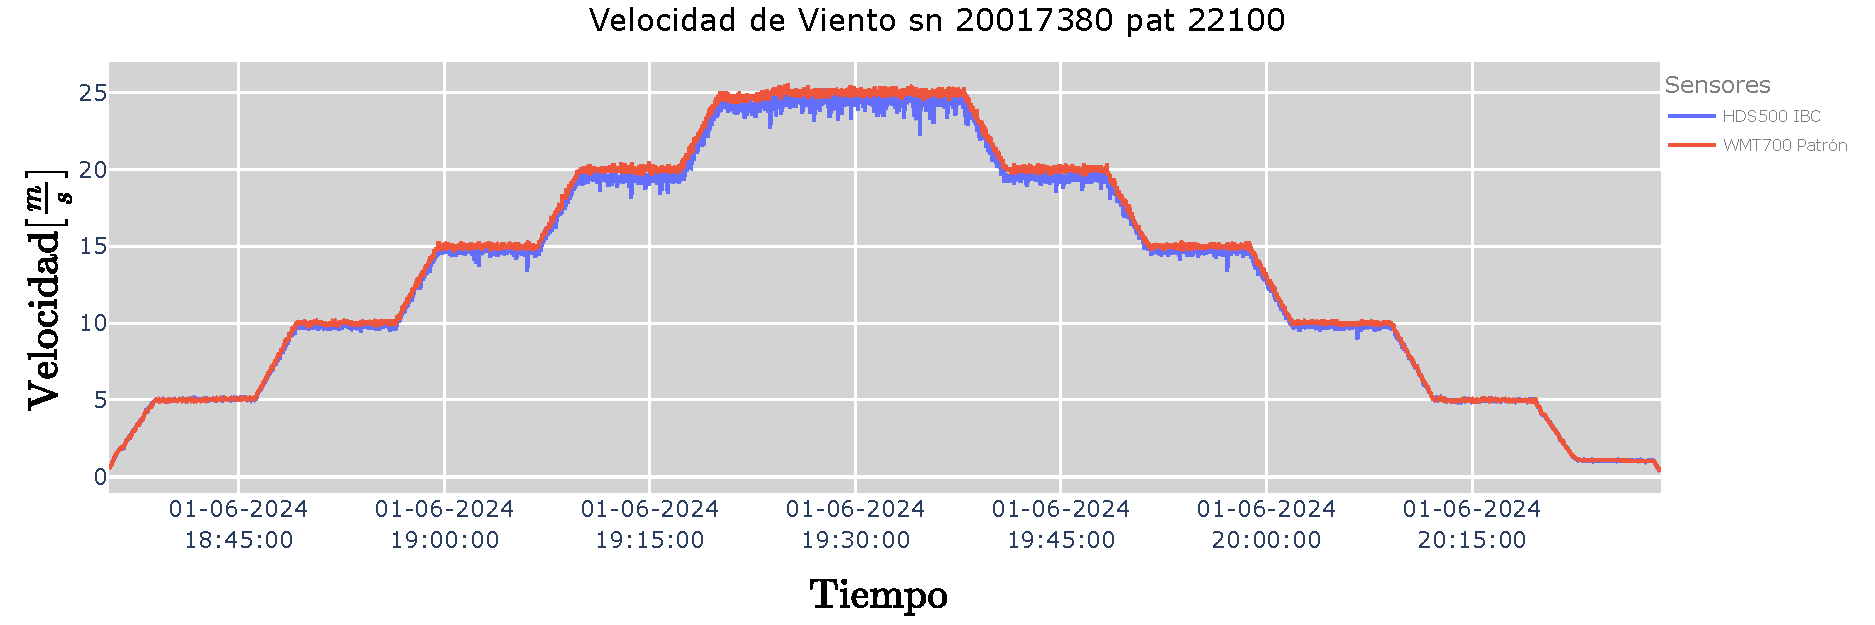
\includegraphics[width=\textwidth]{Figuras/resultados/calibracion/HD51_3/Velocidad de Viento crudo sn 20017380 pat 22100.pdf}}
    \end{minipage}  
    \hspace{2em} % Espacio vertical entre las filas
    \begin{minipage}[b]{1\textwidth}
        \centering
        \subcaptionbox{\label{fig:deltaDireccionCrudo}}{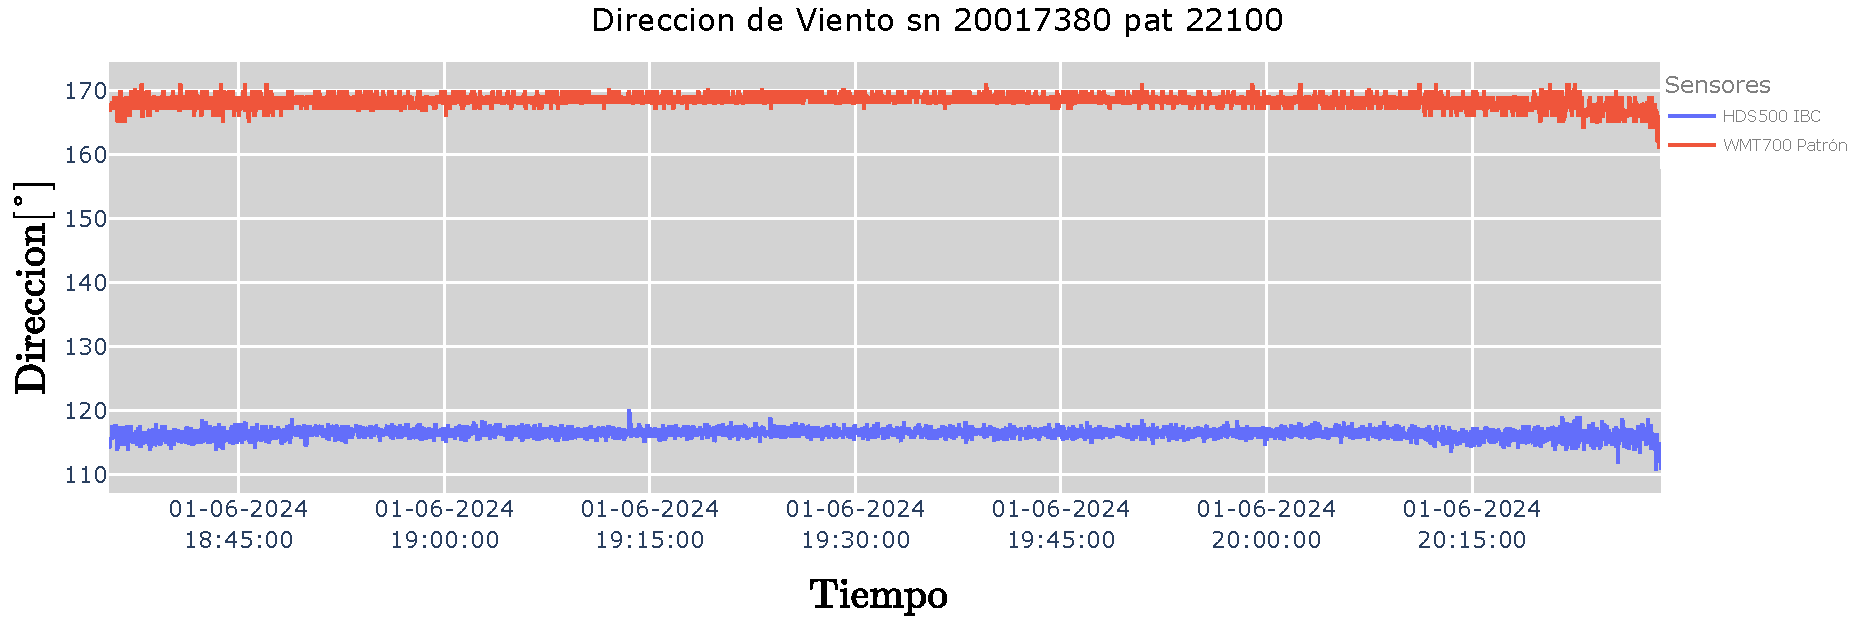
\includegraphics[width=\textwidth]{Figuras/resultados/calibracion/HD51_3/Direccion de Viento sn crudo 20017380 pat 22100.pdf}}
    \end{minipage}  
    \caption{En (a) se muestra el ciclo ascendente y descendente de la velocidad de viento y en (b) se observa la dirección de viento.}
    \label{fig:deltaDatosCrudos}
\end{figure}

A partir de la resta entre los valores promedio del ciclo ascendente y los valores promedio del ciclo descendente, se calcula la histéresis para cada punto. Tomando todos estos puntos, se puede construir una curva de histéresis como se muestra en la Figura \ref{fig:deltaGraficoHister}. En la misma se representan dos regresiones lineales: uno para el ciclo ascendente y otro para el ciclo descendente. Gráficamente, se puede observar que ambas curvas difieren sutilmente y presentan la misma pendiente, con una leve diferencia de 3 centésimos en la ordenada al origen. Además, presentan un factor de correlación cercano a 1, lo que indica que el instrumento presenta muy poca alinealidad, de tal manera que cuando cambia de un valor en ascenso o descenso, lo hace por la misma curva. En la tabla de la Figura \ref{fig:deltaTablaHister} se observa el resultado numérico de la histéresis para cada punto, tanto del patrón como del IBC.

\begin{figure}[H]
    \centering
    \begin{minipage}[b]{1\textwidth}
        \centering
        \subcaptionbox{\label{fig:deltaGraficoHister}}{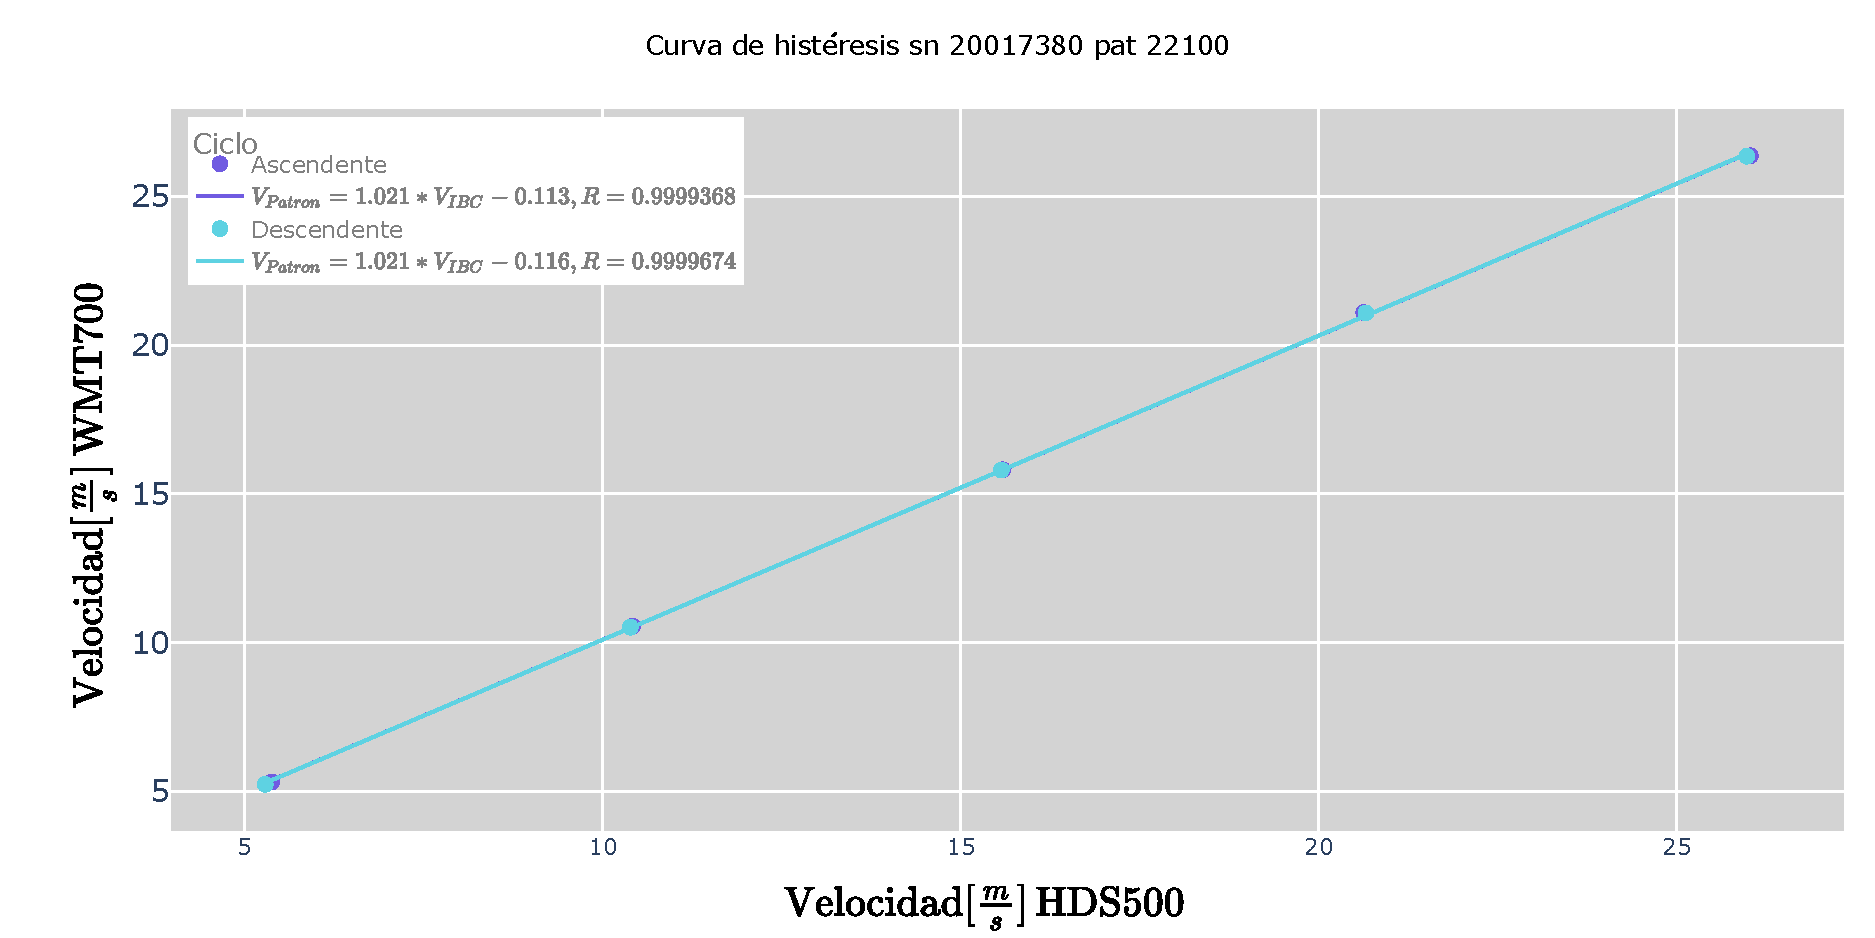
\includegraphics[width=\textwidth]{Figuras/resultados/calibracion/HD51_3/Curva de histeresis sn 20017380 pat 22100.pdf}}
    \end{minipage}  
    \hspace{1em} % Espacio vertical entre las filas
    \begin{minipage}[b]{0.55\textwidth}
        \centering
        \subcaptionbox{\label{fig:deltaTablaHister}}{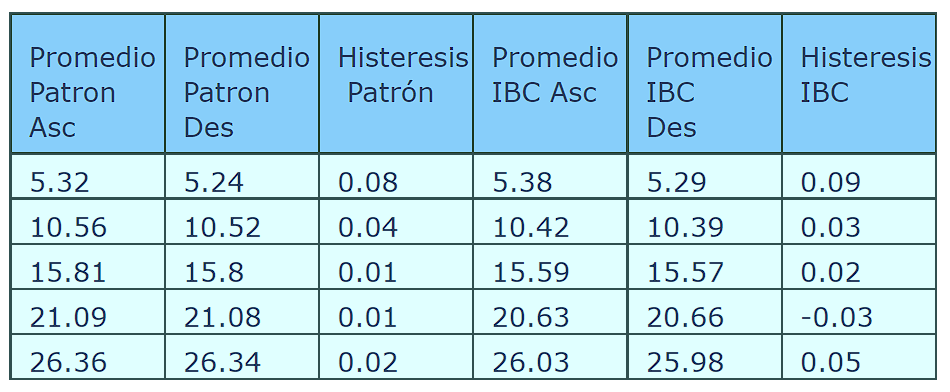
\includegraphics[width=\textwidth]{Figuras/resultados/calibracion/HD51_3/tablaHisteresis.png}}
    \end{minipage}  
    \caption{En (a) se muestra la curva de histéresis para el sensor bajo calibración y en (b) se observa la tabla con los resultados numéricos.}
    \label{fig:deltaResultHisteresis}
\end{figure} 

En la Figura \ref{fig:deltaGraficoCalibAsc} se presenta la curva de calibración, donde los datos del patrón han sido ajustados conforme a su certificado de calibración y comparados con los valores obtenidos mediante el IBC. Adicionalmente, en cada punto se incluye la incertidumbre expandida con un factor de cobertura aproximado de 2. De esta manera, se observa que el ajuste lineal de esta curva se encuentra dentro de los intervalos de incertidumbre, lo que permite afirmar que las mediciones verdaderas se encuentran en dicho intervalo con un nivel de confianza del 95\%. En la leyenda se muestra la función de calibración que se puede utilizar para aplicar las correcciones a las mediciones del IBC mediante software. En caso de que se deban ingresar manualmente las correcciones para el sensor bajo calibración, se proporciona una tabla en la Figura \ref{fig:deltaTablaCalibAsc}, que además cuenta con información de la incertidumbre combinada, la incertidumbre expandida y los grados de libertad. Toda esta información debe ser incluida en el certificado de calibración del IBC.


\begin{figure}[H]
    \centering
    \begin{minipage}[b]{1\textwidth}
        \centering
        \subcaptionbox{\label{fig:deltaGraficoCalibAsc}}{\includegraphics[width=\textwidth]{Figuras/resultados/calibracion/HD51_3/Curva de calibración Asc sn 20017380 pat 22100.pdf}}
    \end{minipage}  
    \hspace{1em} % Espacio vertical entre las filas
    \begin{minipage}[b]{0.7\textwidth}
        \centering
        \subcaptionbox{\label{fig:deltaTablaCalibAsc}}{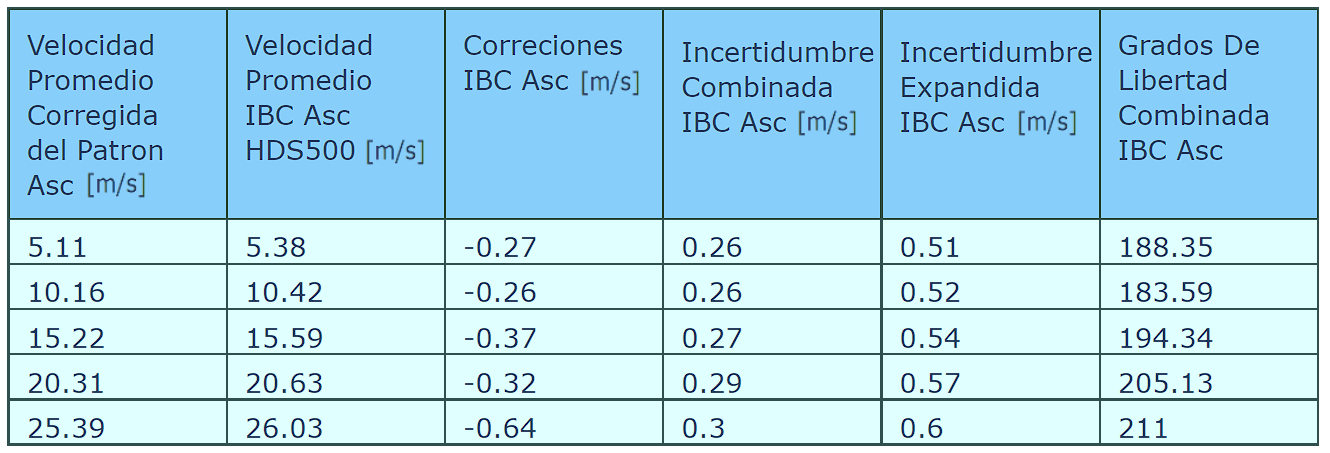
\includegraphics[width=\textwidth]{Figuras/resultados/calibracion/HD51_3/tablaResultadosAsc.png}}
    \end{minipage}  
    \caption{En (a) se presenta la curva de calibración ascendente con sus respectivas incertidumbres expandidas, y en (b) se muestra la tabla con los resultados numéricos.}
    \label{fig:deltaResultCalibAsc}
\end{figure} 

Para las mediciones del ciclo descendente también se cuenta con una curva de calibración, Figura \ref{fig:deltaGraficoCalibDes}, la cual se puede utilizar para proporcionar información sobre la incertidumbre con la que se trabaja y aplicar las correcciones a las mediciones del instrumento. En la tabla de la Figura \ref{fig:deltaTablaCalibDes} también se muestran los resultados de esta calibración.

\begin{figure}[H]
    \centering
    \begin{minipage}[b]{1\textwidth}
        \centering
        \subcaptionbox{\label{fig:deltaGraficoCalibDes}}{\includegraphics[width=\textwidth]{Figuras/resultados/calibracion/HD51_3/Curva de calibración Des sn 20017380 pat 22100.pdf}}
    \end{minipage}  
    \hspace{2em} % Espacio vertical entre las filas
    \begin{minipage}[b]{0.7\textwidth}
        \centering
        \subcaptionbox{\label{fig:deltaTablaCalibDes}}{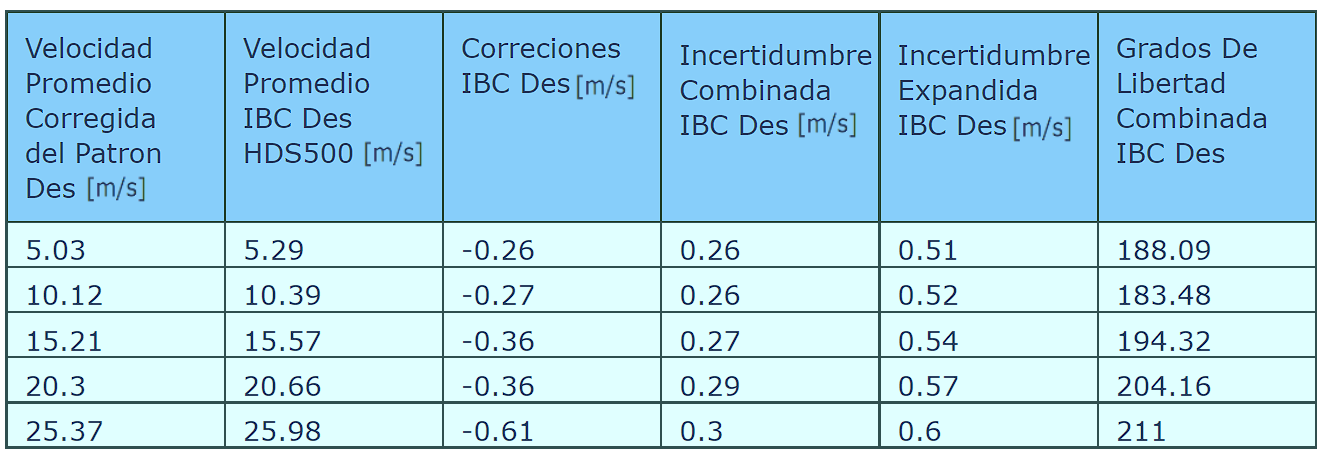
\includegraphics[width=\textwidth]{Figuras/resultados/calibracion/HD51_3/tablasResultadosDesc.png}}
    \end{minipage}  
    \caption{En (a) se presenta la curva de calibración descendente con sus respectivas incertidumbres expandidas, y en (b) se muestra la tabla con los resultados numéricos.}
    \label{fig:deltaResultCalibDes}
\end{figure} 

La información que se incluye en el certificado de calibración puede contener las dos curvas de calibración, tanto ascendente como descendente, o solo una de ellas. También es posible proporcionar únicamente alguna de las tablas de calibración, permitiendo que el usuario final realice una regresión lineal de los puntos y determine su propia curva de calibración. No obstante, el laboratorio no realiza el ajuste del instrumento, y la decisión final recae en el usuario final. En particular, los instrumentos que maneja el SMN tienen tolerancias máximas para cada magnitud física \cite{wmo2020} establecidas por la WMO. Para la variable viento se acepta una incertidumbre de $\pm \SI{1}{\meter\per\second}$ para ser considerado un instrumento de clase A, una incertidumbre de $\pm \SI{2}{\meter\per\second}$ para ser considerado de clase B, o una incertidumbre de $\pm \SI{5}{\meter\per\second}$ para ser considerado de clase C. Dependiendo de la categoría, el instrumento podrá ser utilizado para distintas aplicaciones.


%%%%%%%%%%%%%%%%%%%%%%%%%%%%%%%%%%%%%%%%%%%%%%%%%%%%%%%%%%%%%%%%%%%%%%%%%%%%%%%%%%%%%%%%%%%%%%%%%%%%%%%%%%%%%%%%%%%%%%%%
% \section{Calibración Vaisala WMT700}\label{sec:calibVaisala}

% \subsection{Banco de medición y configuración del hardware}\label{sec:bancoMedicionVaisala}

% En la Figura \ref{fig:deltaVistaFrontal} se muestra en (a) el montaje de los sensores sobre una barra de acero, de la misma forma que el caso anterior se tiene  distancia $d$ de \SI{65}{\centi\meter} y a una altura $h$ respecto a la base del soporte de \SI{36.5}{\centi\meter}. Los sensores quedan alineados y nivelados en el eje longitudinal de la barra, como se muestra en las Figuras \ref{fig:deltaVistaSup2} y \ref{fig:deltaVistaPerfil}.


% \begin{figure}[H]
%     \centering
%     \begin{minipage}[b]{0.6\textwidth}
%         % \centering
%         \subcaptionbox{\label{fig:vaisalaVistaFrontal}}{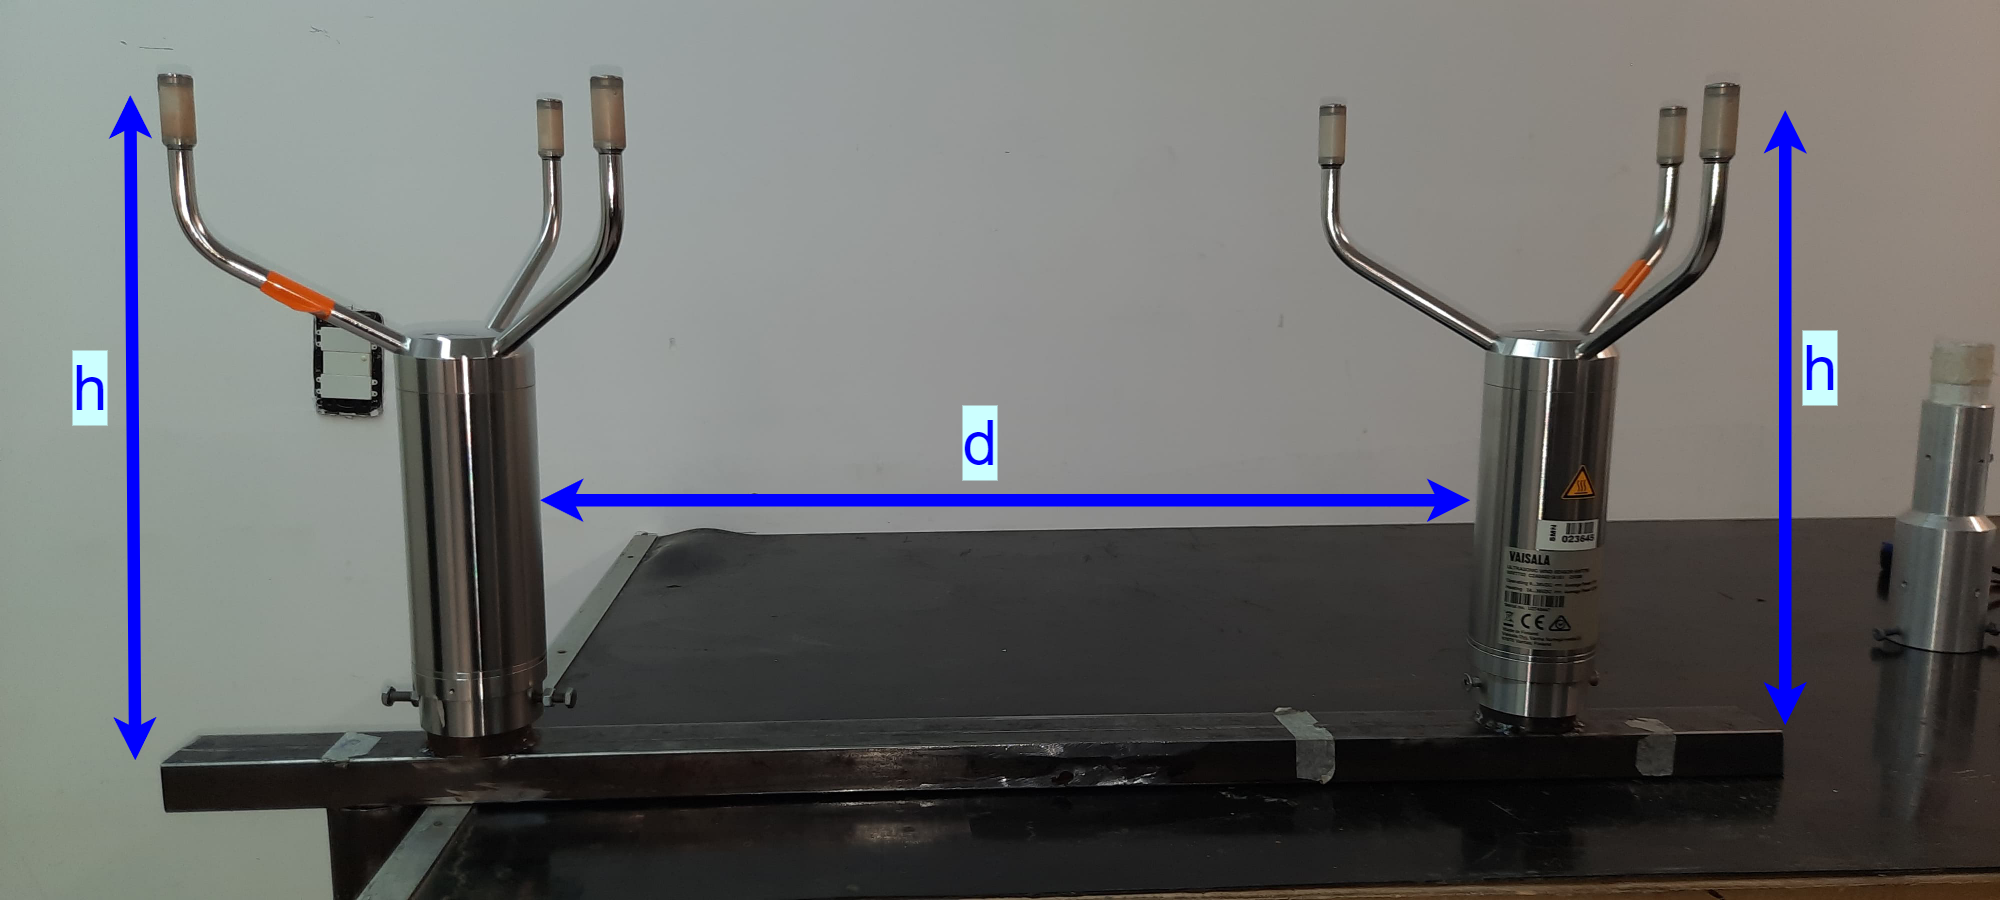
\includegraphics[width=\textwidth]{Figuras/resultados/calibracion/WMT700/vaisalaVistaFrontal.png}}
%         \subcaptionbox{\label{fig:vaisalaVistaSup}}{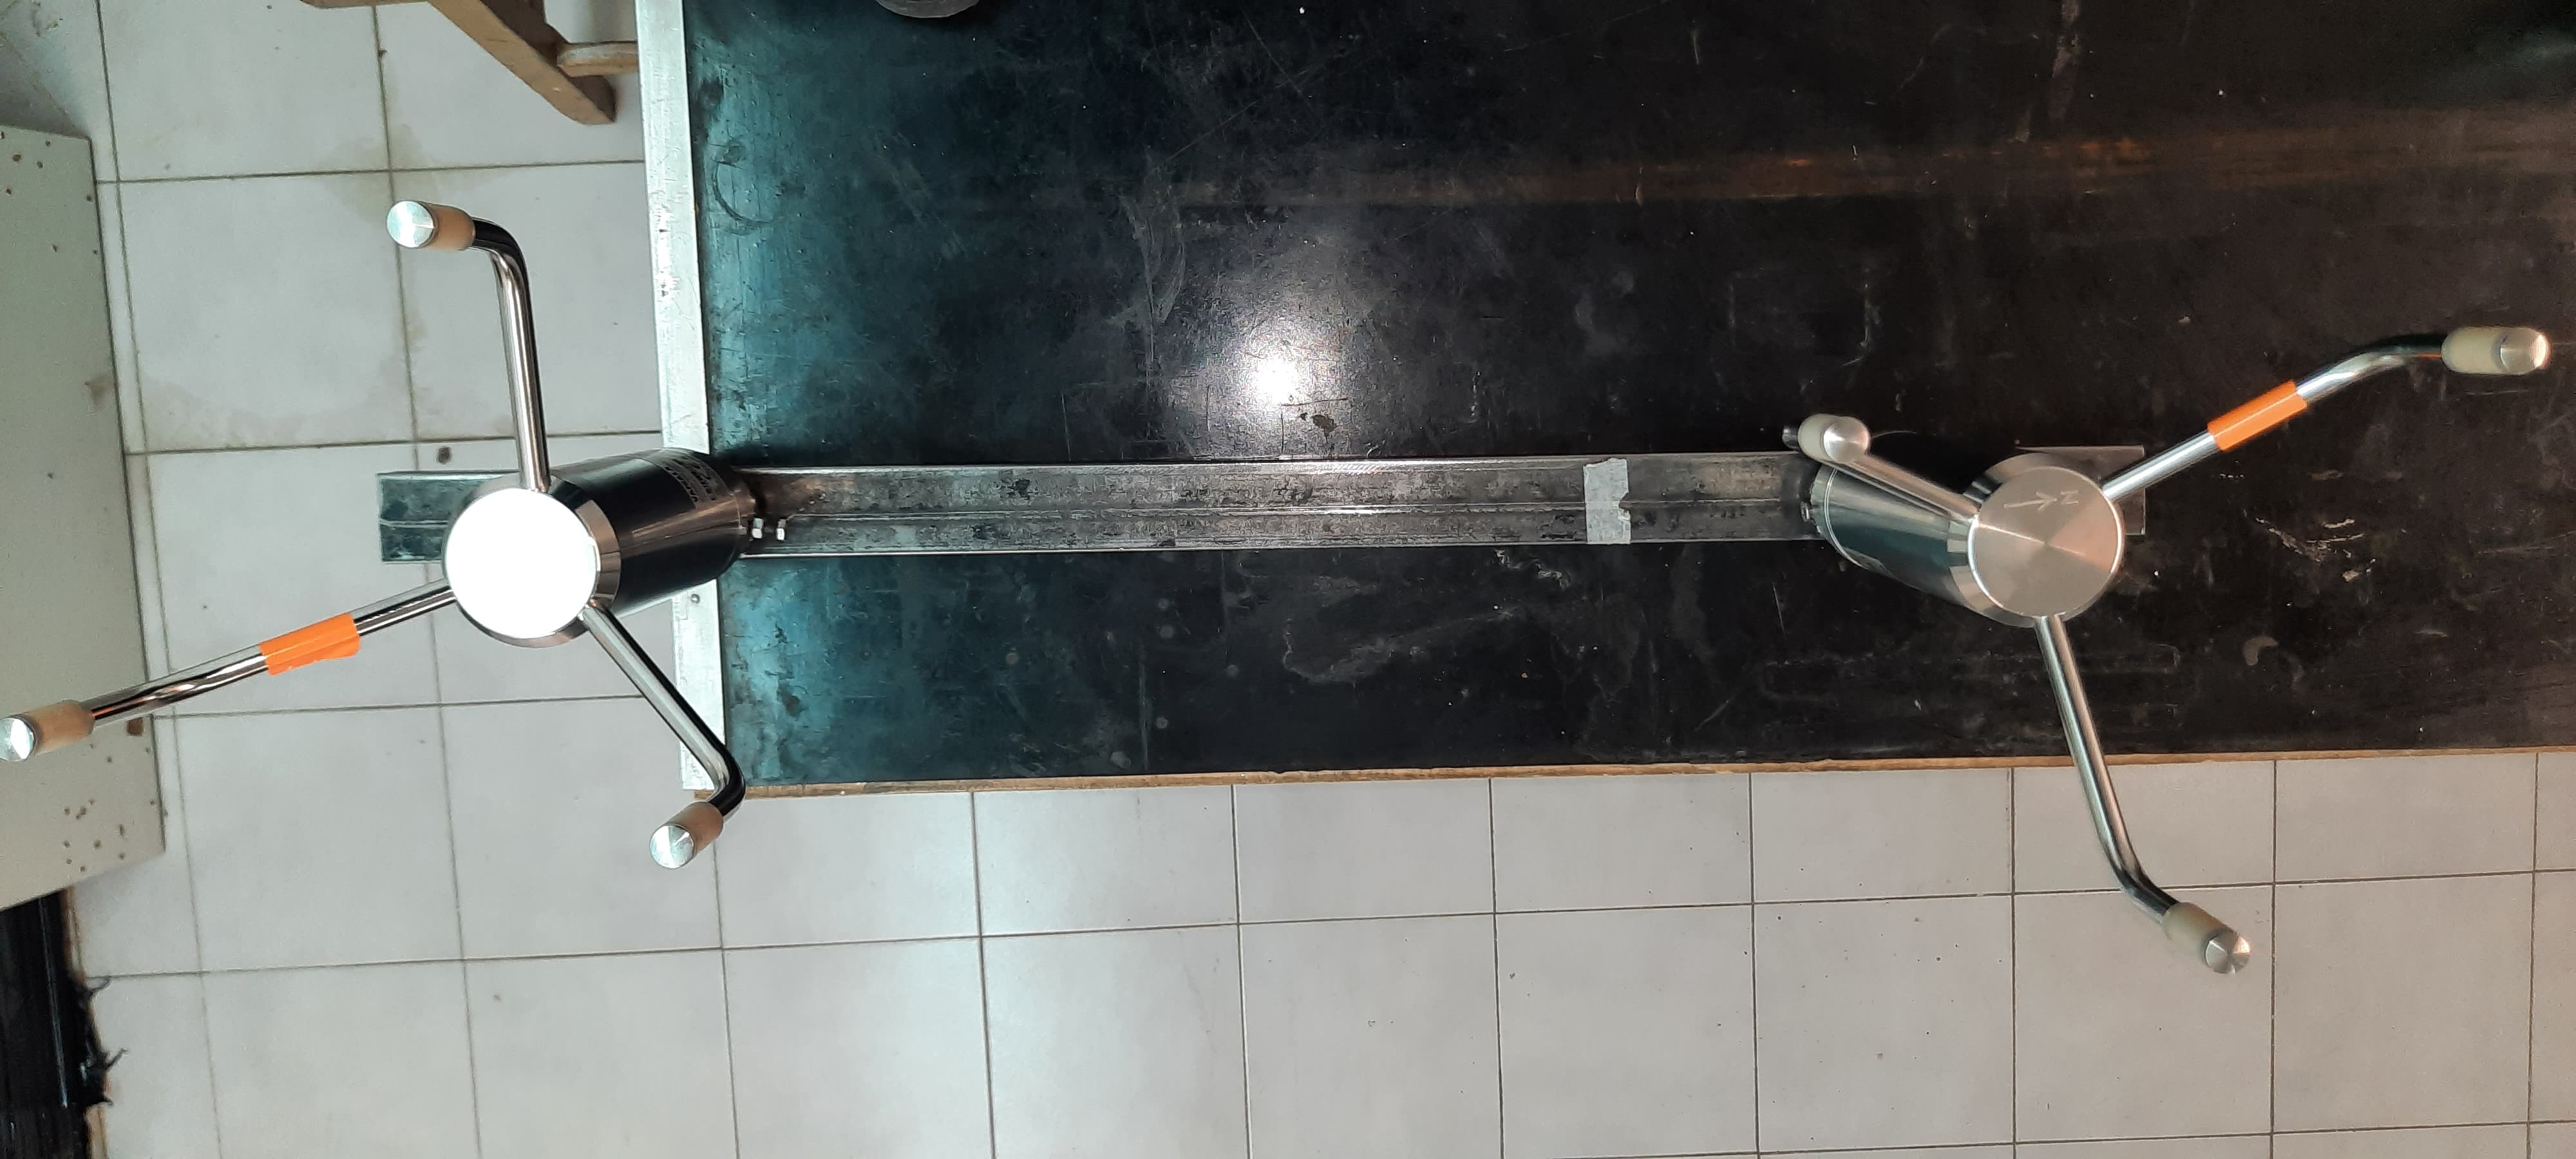
\includegraphics[width=\textwidth]{Figuras/resultados/calibracion/WMT700/vaisalaVistaSup.jpg}}
%     \end{minipage}  
%     \hspace{1em} % Espacio vertical entre las filas
%     \begin{minipage}[b]{0.25\textwidth}
%         % \centering
%         \subcaptionbox{\label{fig:vaisalaVistaPerfil3}}{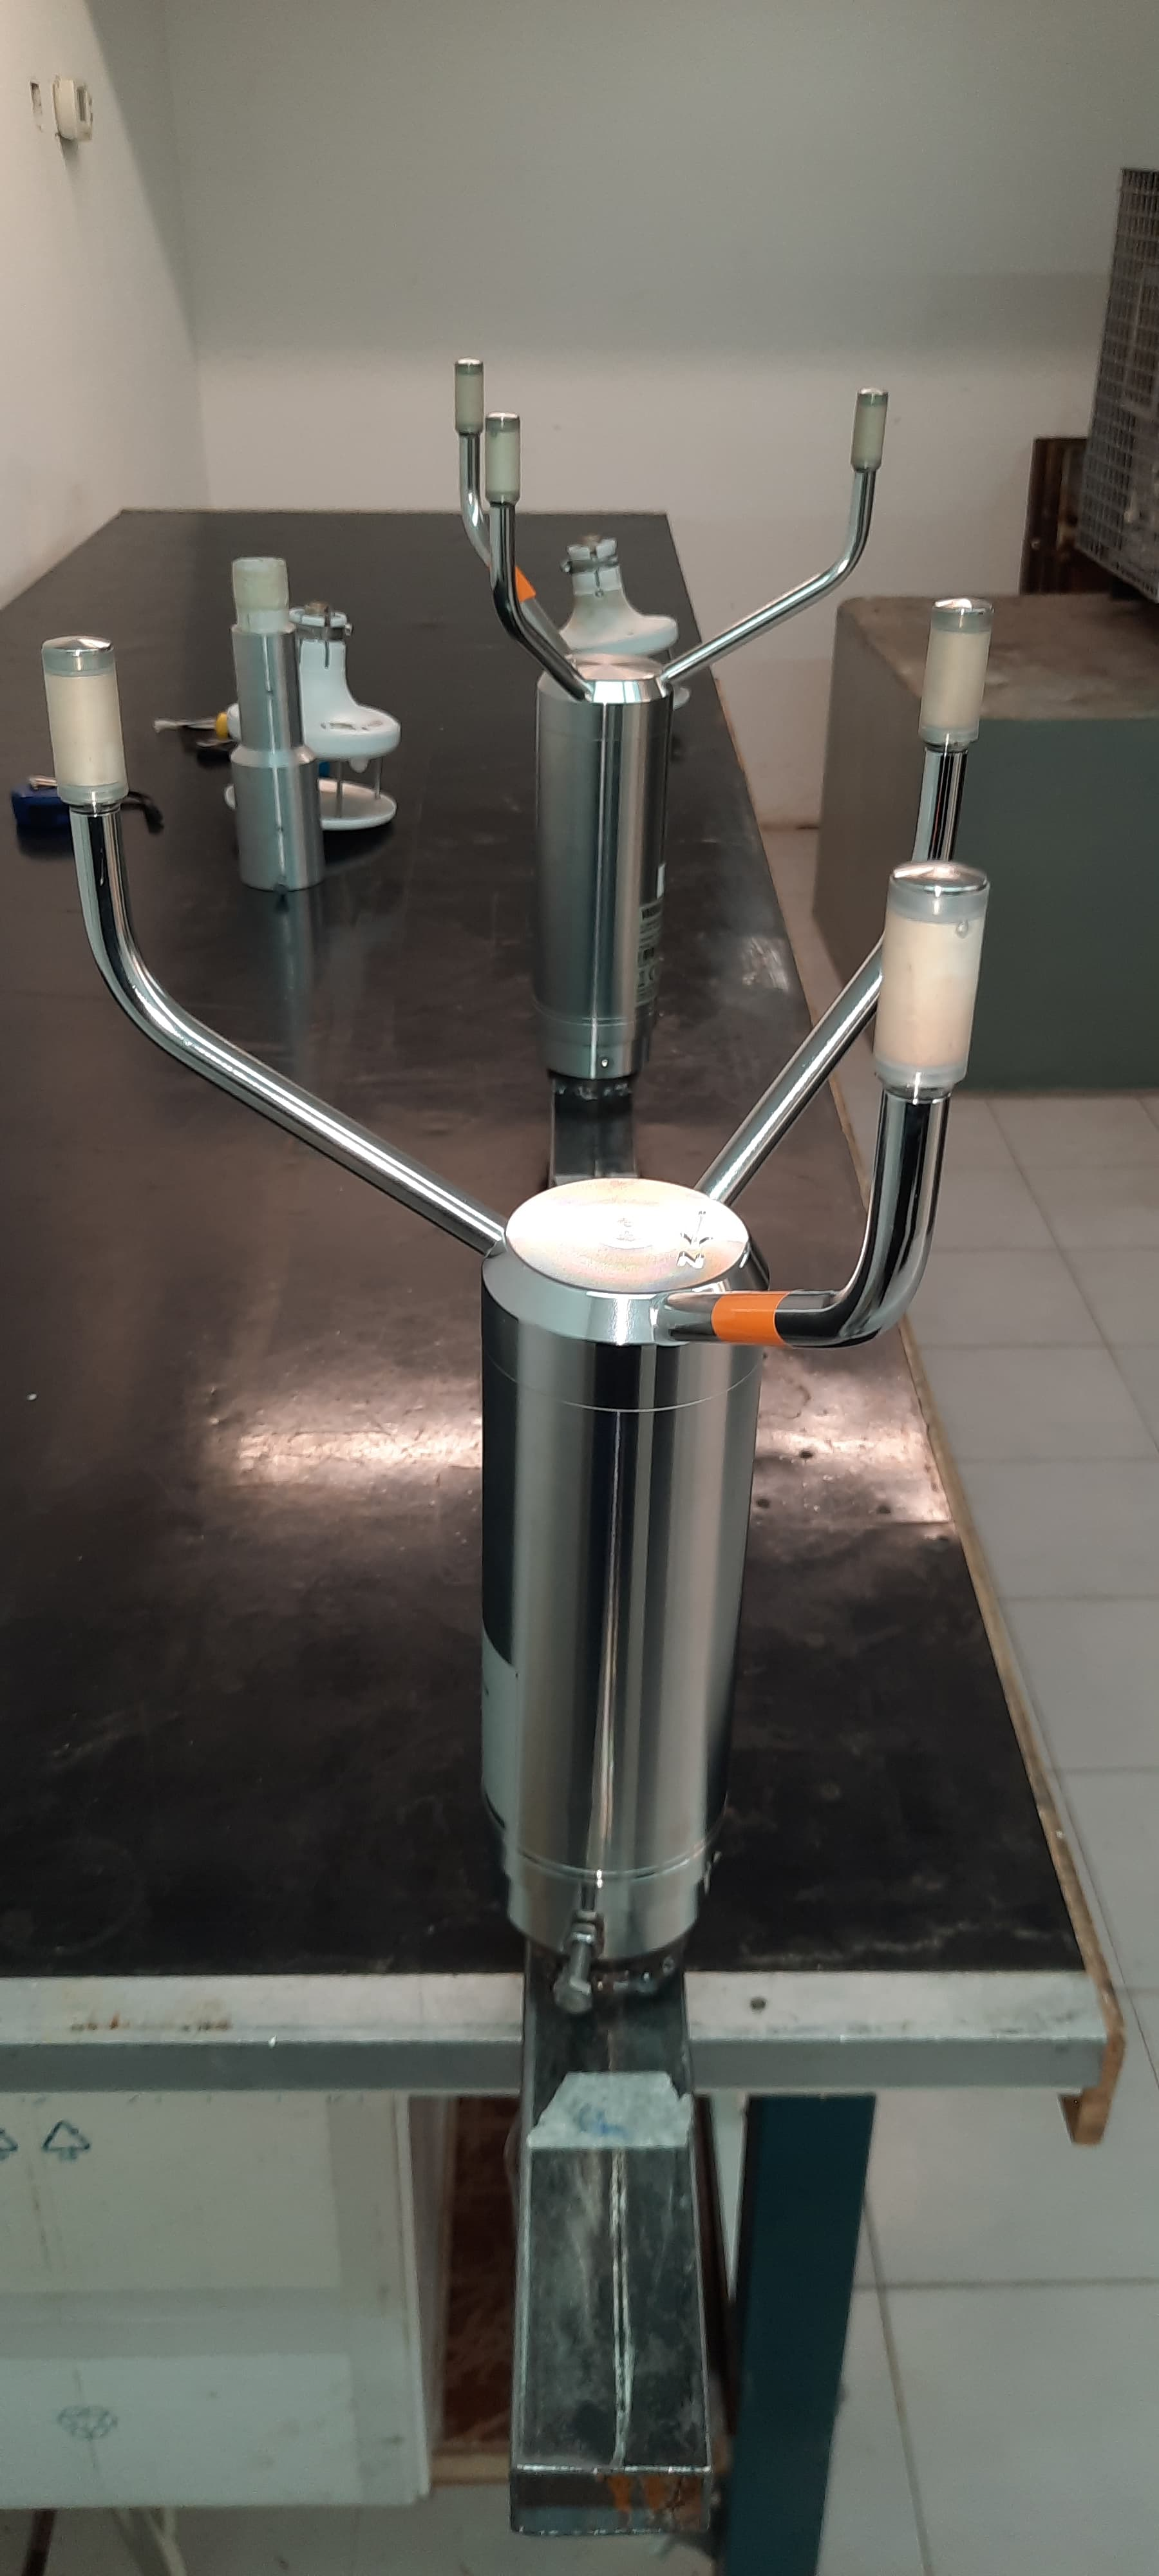
\includegraphics[width=\textwidth]{Figuras/resultados/calibracion/WMT700/vaisalaVistaPerfil3.jpg}}
%     \end{minipage}
%     \caption{En (a) se muestra  , en (b)  y en (c) .}
%     \label{fig:bancoMedicionVaisala}
% \end{figure} 


% Sensor montado en el tunel de viento en lal Figura \ref{fig:vaisaldaMontajeTunel}. Se utiliza la misma mesa de trabajo de la figura \ref{fig:vaisaldaMontajeTunel}, donde solo se cambio el sensor HD51.3 por otro sensor WMT700.
% \begin{figure}[H]
%     \centering
%     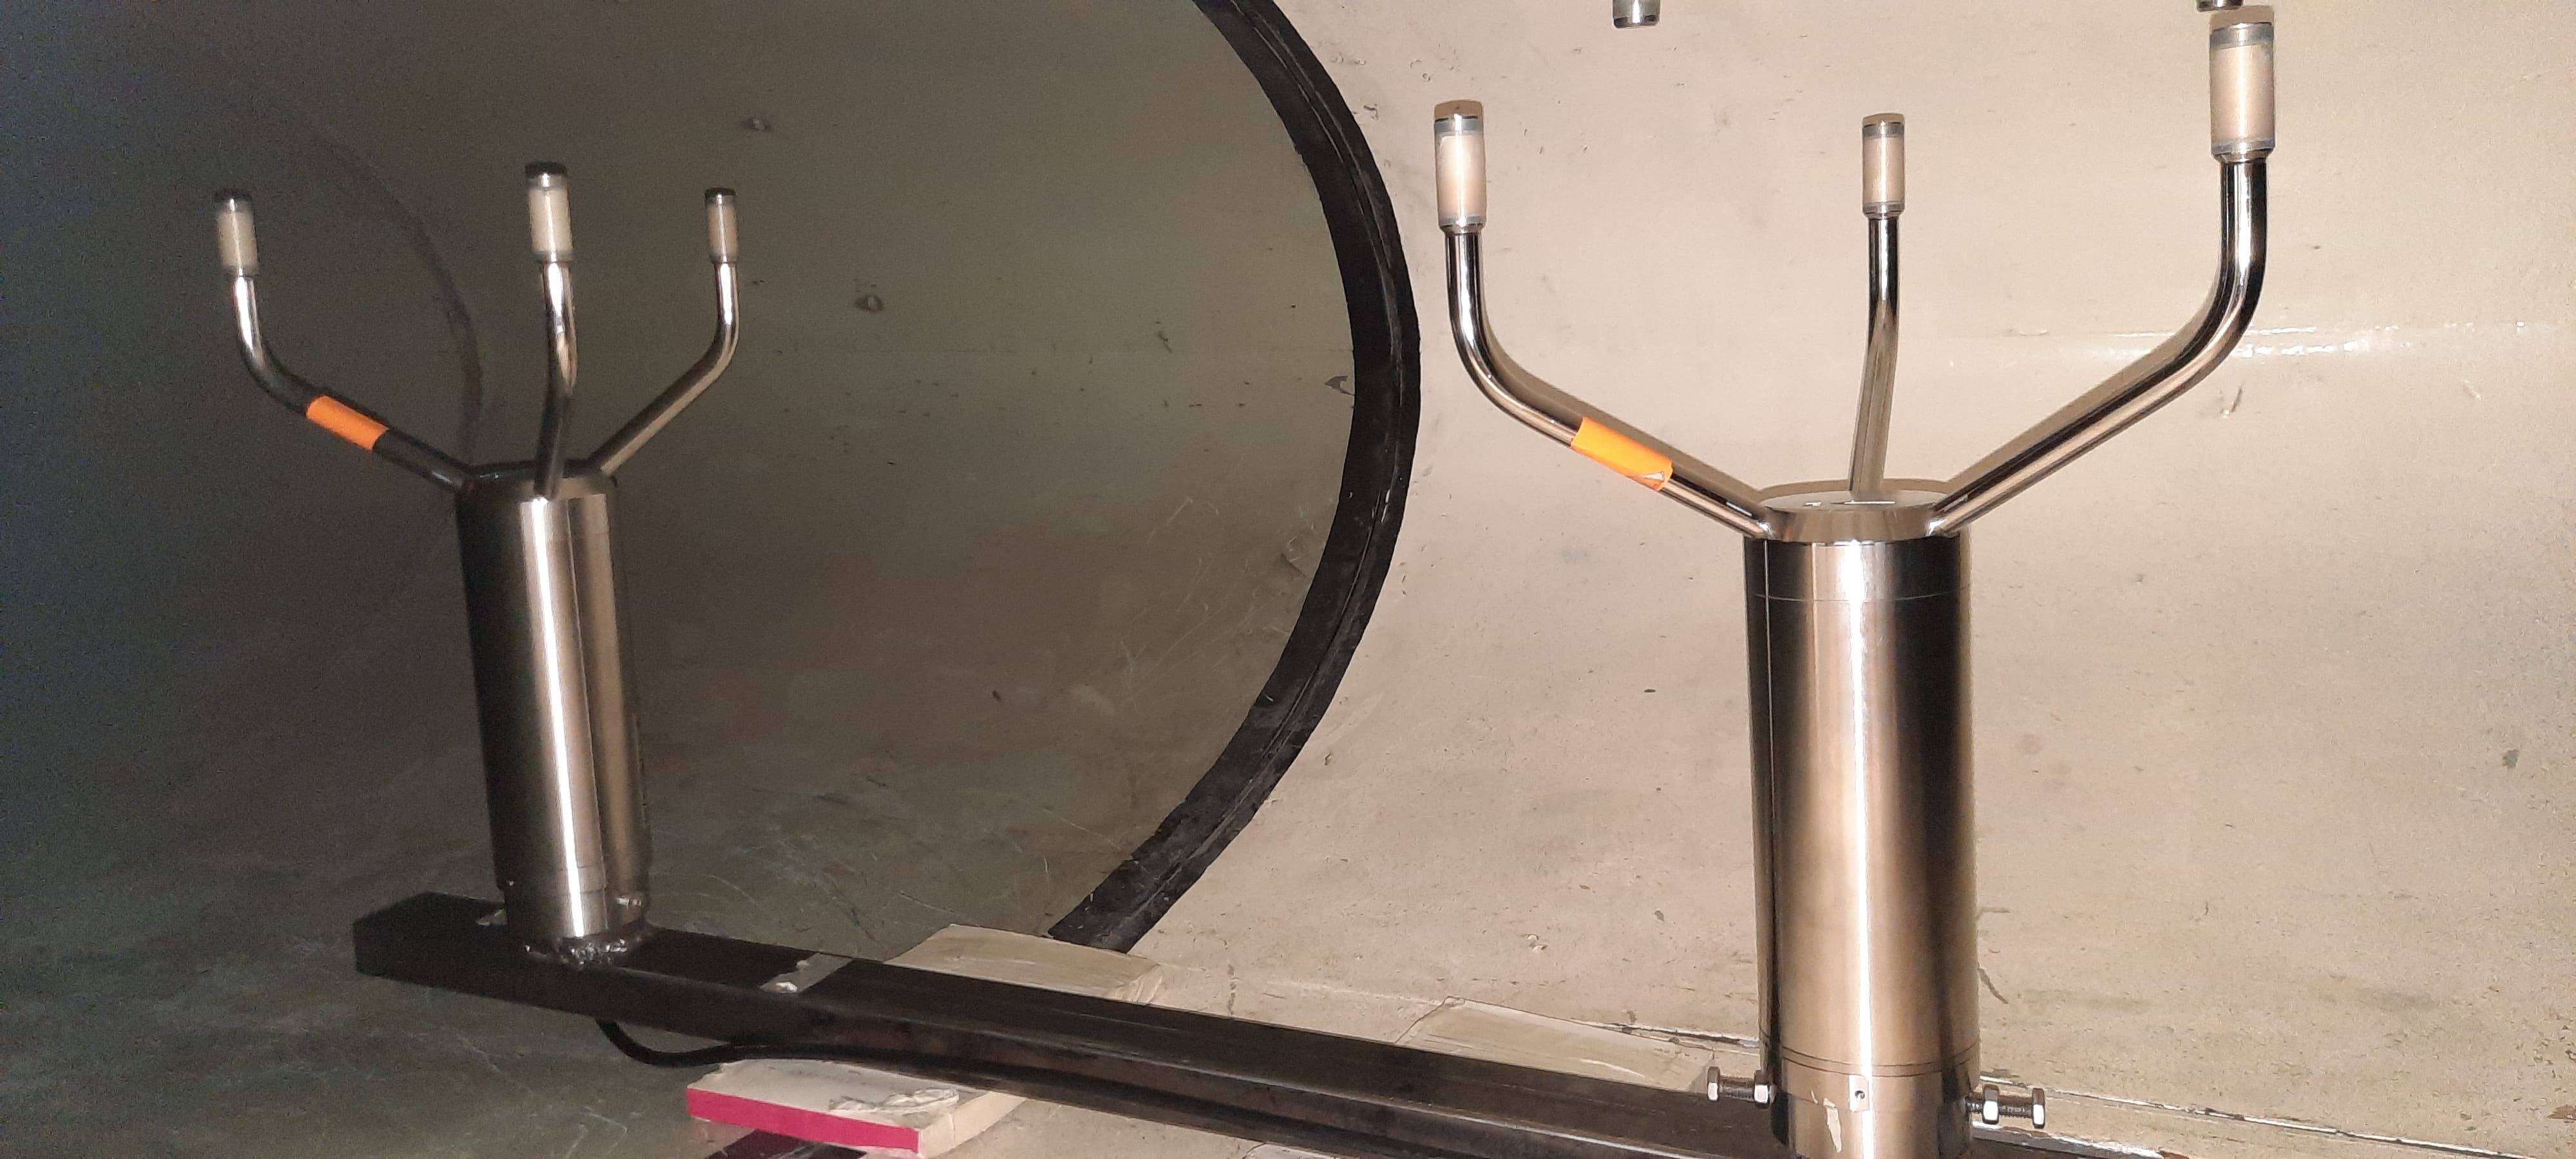
\includegraphics[width=0.7\linewidth]{Figuras/resultados/calibracion/WMT700/vaisalaMontadoTunel.jpg}
%     \caption{Brazo con los sensores bajo calibración a izquierda y patrón a derecha dentro del túnel.}
%     \label{fig:vaisalaMontadoTunel}
% \end{figure}

% \subsection{Configuración de la aplicación web}
% La configuración del certificado de calibración y certificado del túnel de viento es la misma que las figuras \ref{fig:configDataloggerDelta} y ref{fig:configTunelDelta}, ya que se trabajo con el mismo patron en las mismas condiciones para el túnel.
% \begin{figure}[H]
%     \centering
%     \begin{minipage}[b]{0.2\textwidth}
%         \centering
%         \subcaptionbox{\label{fig:configSensorIBCVaisala}}{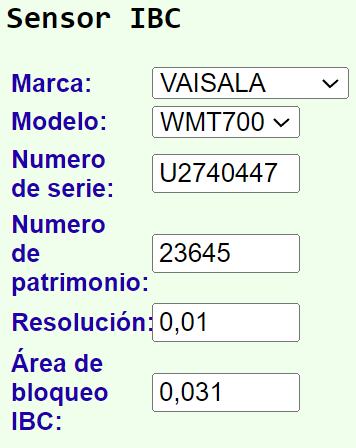
\includegraphics[width=\textwidth]{Figuras/resultados/calibracion/WMT700/configSensorIBC.png}}
%     \end{minipage}  
%     \hspace{1em} % Espacio vertical entre las filas
%     \begin{minipage}[b]{0.18\textwidth}
%         \centering
%         \subcaptionbox{\label{fig:configSensorPATVaisala}}{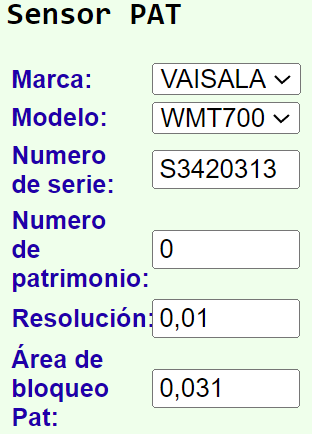
\includegraphics[width=\textwidth]{Figuras/resultados/calibracion/WMT700/configSensorPat.png}}
%     \end{minipage}
%     \caption{En (a) se muestra ...y en (b) se observa}
%     \label{fig:configMetadatosVaisala}
% \end{figure} 


% cofig de los equipos

% \begin{figure}[H]
%     \centering
%     \begin{minipage}[b]{0.2\textwidth}
%         \centering
%         \subcaptionbox{\label{fig:configDataloggerVaisala}}{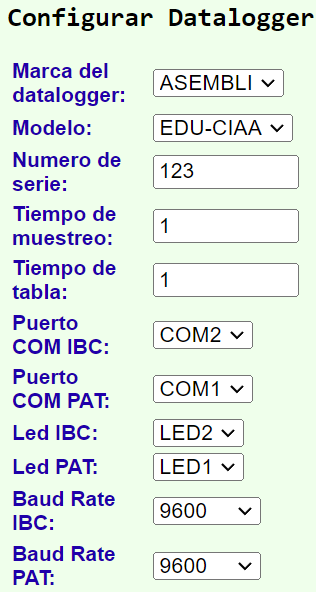
\includegraphics[width=\textwidth]{Figuras/resultados/calibracion/WMT700/configDatalogger.png}}
%     \end{minipage}  
%     \hspace{1em} % Espacio vertical entre las filas
%     \begin{minipage}[b]{0.22\textwidth}
%         \centering
%         \subcaptionbox{\label{fig:configTunelVaisala}}{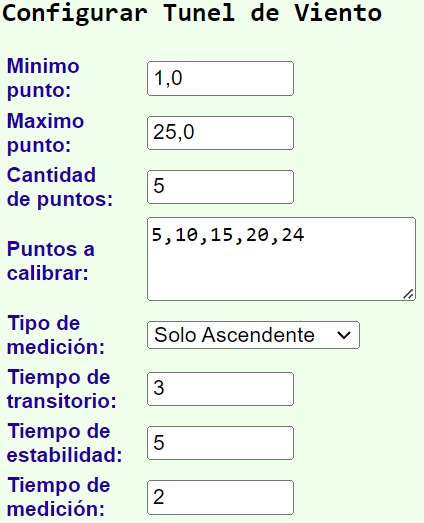
\includegraphics[width=\textwidth]{Figuras/resultados/calibracion/WMT700/configTunel.png}}
%     \end{minipage}  
%     \caption{En (a) se muestra ...y en (b) se observa ... .}
%     \label{fig:configEquiposVaisala}
% \end{figure} 


% \subsection{Resultados}

% \begin{figure}[H]
%     \centering
%     \begin{minipage}[b]{1\textwidth}
%         \centering
%         \subcaptionbox{\label{fig:vaisalaVelocidadCrudo}}{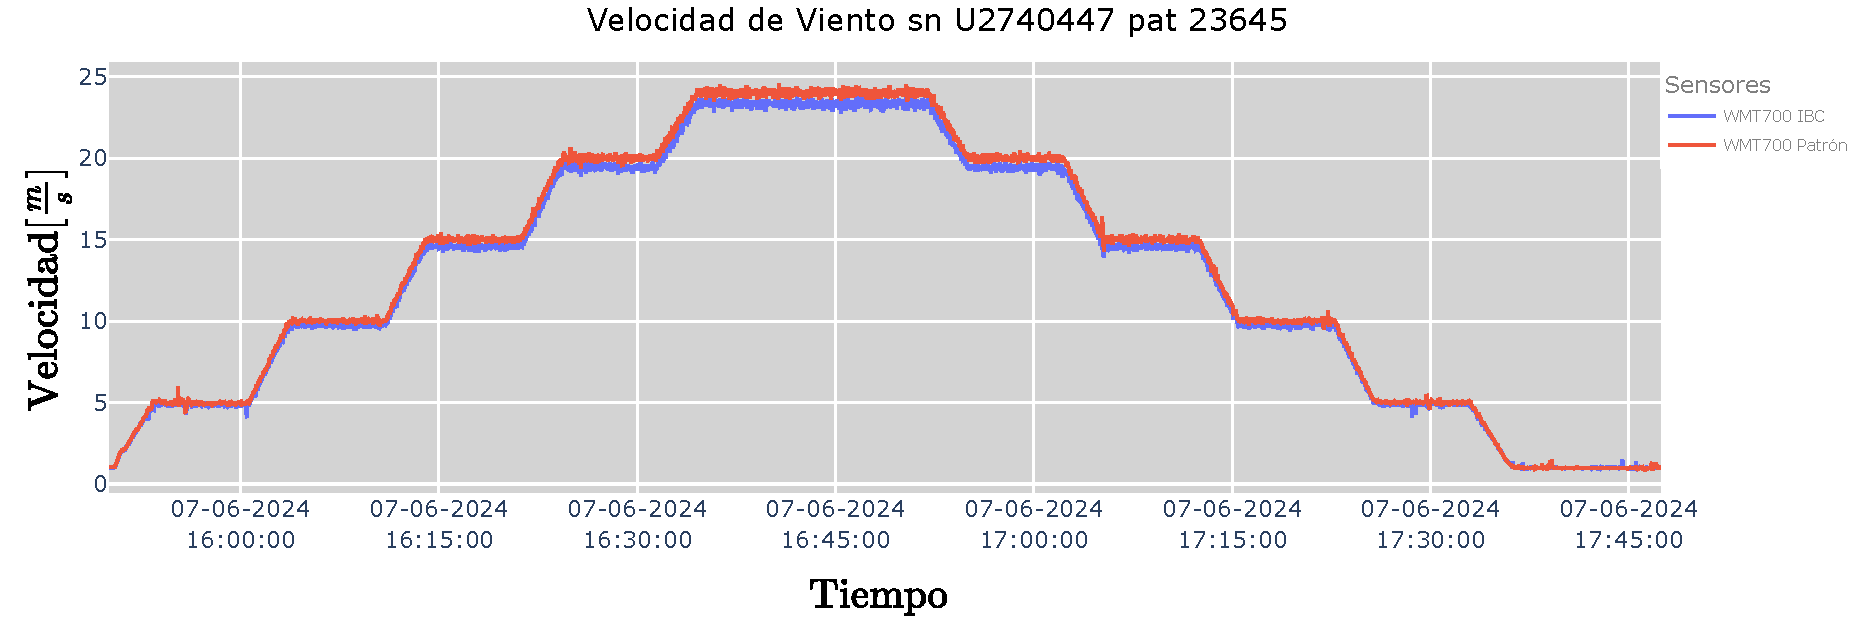
\includegraphics[width=\textwidth]{Figuras/resultados/calibracion/WMT700/Velocidad de Viento sn U2740447 pat 23645.pdf}}
%     \end{minipage}  
%     \hspace{2em} % Espacio vertical entre las filas
%     \begin{minipage}[b]{1\textwidth}
%         \centering
%         \subcaptionbox{\label{fig:vaisalaDireccionCrudo}}{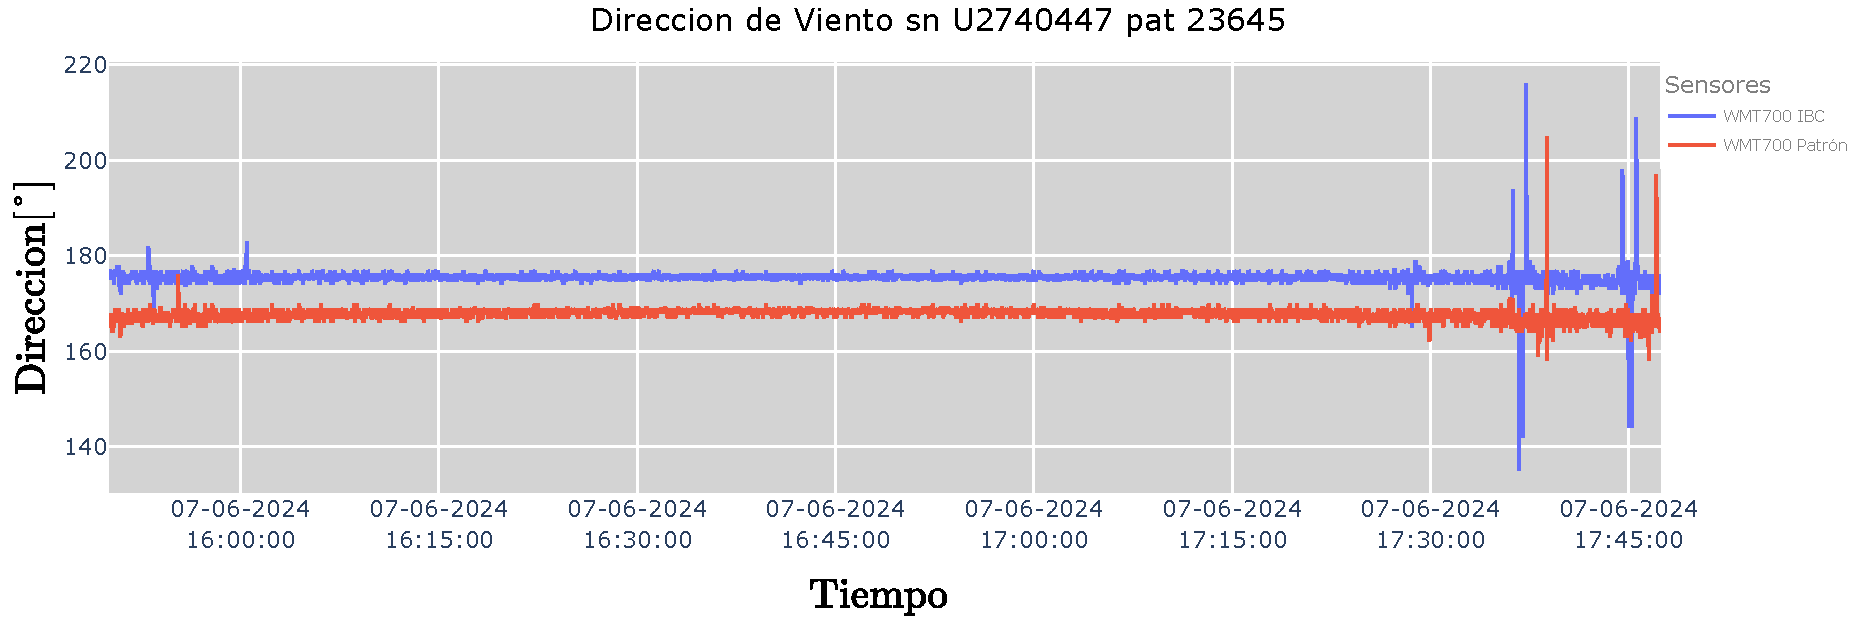
\includegraphics[width=\textwidth]{Figuras/resultados/calibracion/WMT700/Direccion de Viento sn U2740447 pat 23645.pdf}}
%     \end{minipage}  
%     \caption{En (a) se muestra ...y en (b) se observa ... .}
%     \label{fig:vaisalaDatosCrudos}
% \end{figure}

% \begin{figure}[H]
%     \centering
%     \begin{minipage}[b]{1\textwidth}
%         \centering
%         \subcaptionbox{\label{fig:vaisalaGraficoHister}}{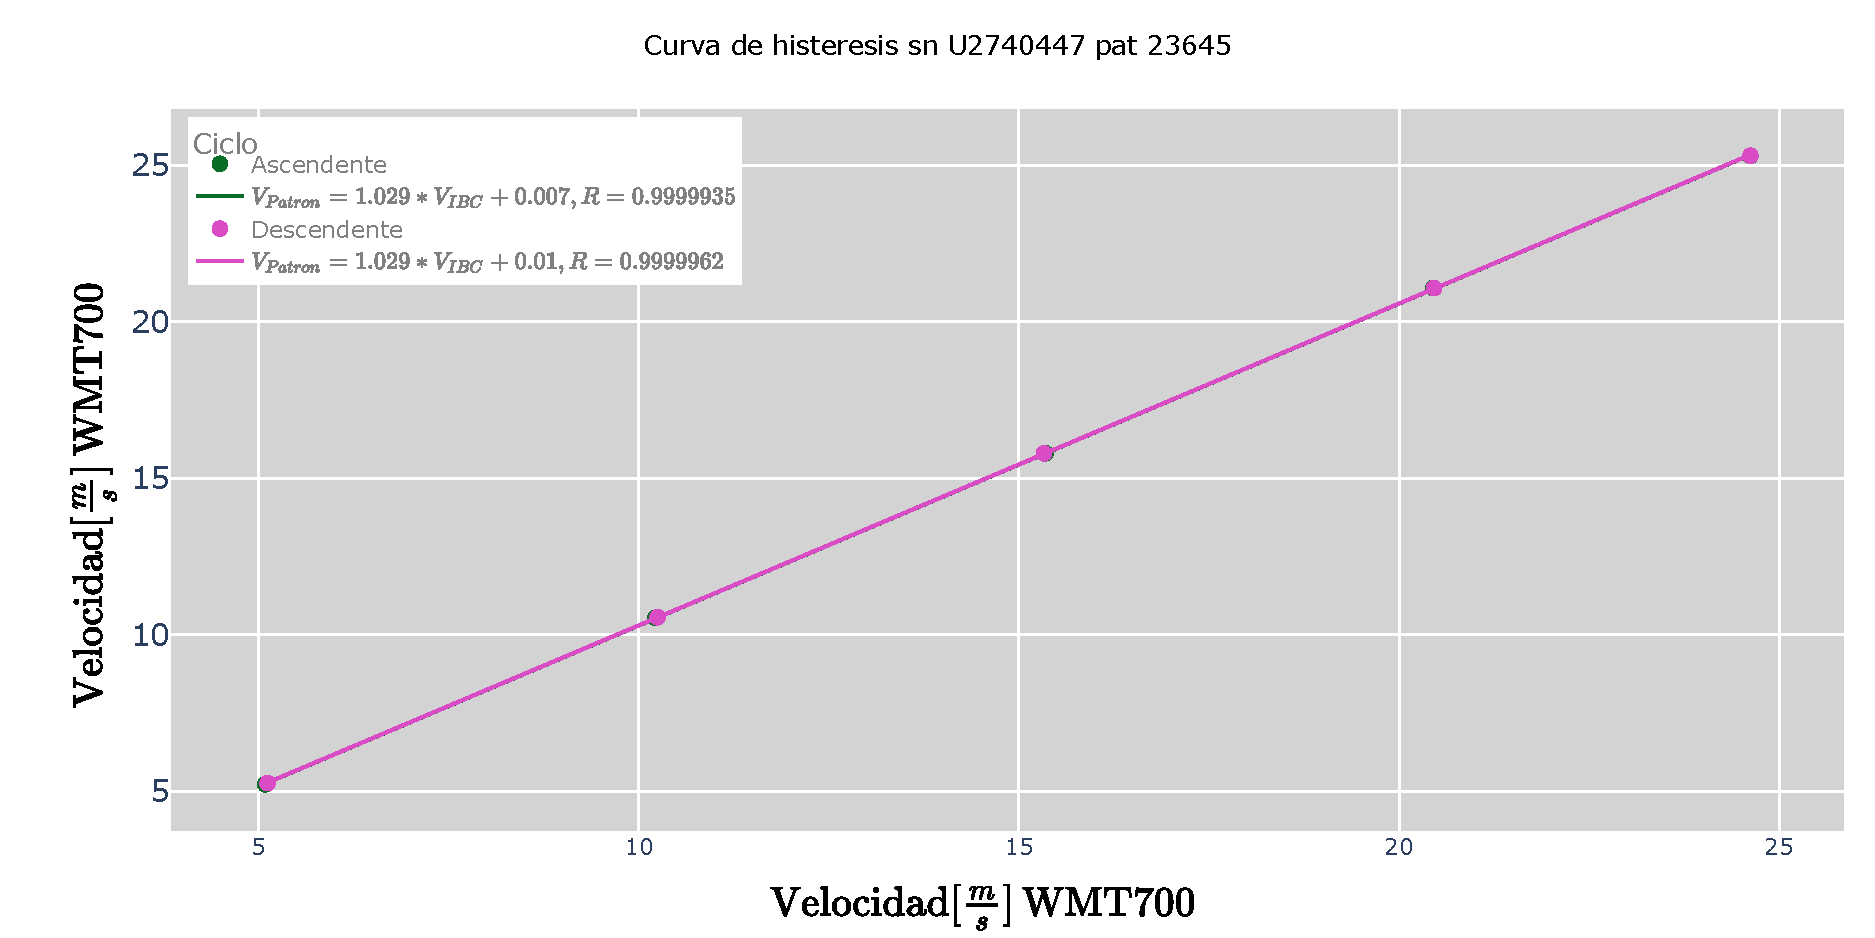
\includegraphics[width=\textwidth]{Figuras/resultados/calibracion/WMT700/Curva de histeresis sn U2740447 pat 23645.pdf}}
%     \end{minipage}  
%     \hspace{1em} % Espacio vertical entre las filas
%     \begin{minipage}[b]{0.55\textwidth}
%         \centering
%         \subcaptionbox{\label{fig:vaisalaTablaHister}}{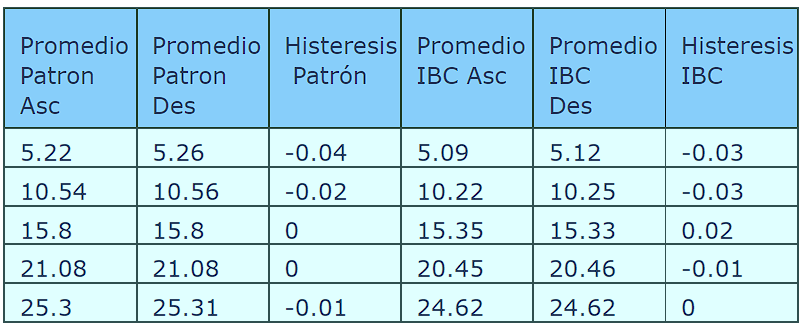
\includegraphics[width=\textwidth]{Figuras/resultados/calibracion/WMT700/tablaVaisalaHisteresis.png}}
%     \end{minipage}  
%     \caption{En (a) se muestra ...y en (b) se observa ... .}
%     \label{fig:vaisalaResultHisteresis}
% \end{figure} 


% \begin{figure}[H]
%     \centering
%     \begin{minipage}[b]{1\textwidth}
%         \centering
%         \subcaptionbox{\label{fig:vaisalaGraficoCalibAsc}}{\includegraphics[width=\textwidth]{Figuras/resultados/calibracion/WMT700/Curva de calibración Asc sn U2740447 pat 23645.pdf}}
%     \end{minipage}  
%     \hspace{1em} % Espacio vertical entre las filas
%     \begin{minipage}[b]{0.7\textwidth}
%         \centering
%         \subcaptionbox{\label{fig:vaisalaTablaCalibAsc}}{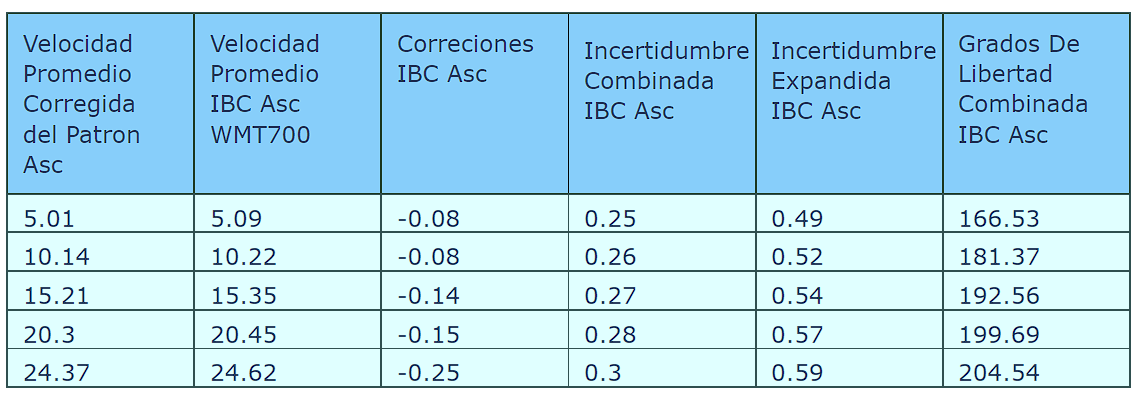
\includegraphics[width=\textwidth]{Figuras/resultados/calibracion/WMT700/tablaVaisalaCalibAsc.png}}
%     \end{minipage}  
%     \caption{En (a) se muestra ...y en (b) se observa ... .}
%     \label{fig:vaisalaResultCalibAsc}
% \end{figure} 


% \begin{figure}[H]
%     \centering
%     \begin{minipage}[b]{1\textwidth}
%         \centering
%         \subcaptionbox{\label{fig:vaisalaGraficoCalibDes}}{\includegraphics[width=\textwidth]{Figuras/resultados/calibracion/WMT700/Curva de calibración Des sn U2740447 pat 23645.pdf}}
%     \end{minipage}  
%     \hspace{2em} % Espacio vertical entre las filas
%     \begin{minipage}[b]{0.7\textwidth}
%         \centering
%         \subcaptionbox{\label{fig:vaisalaTablaCalibDes}}{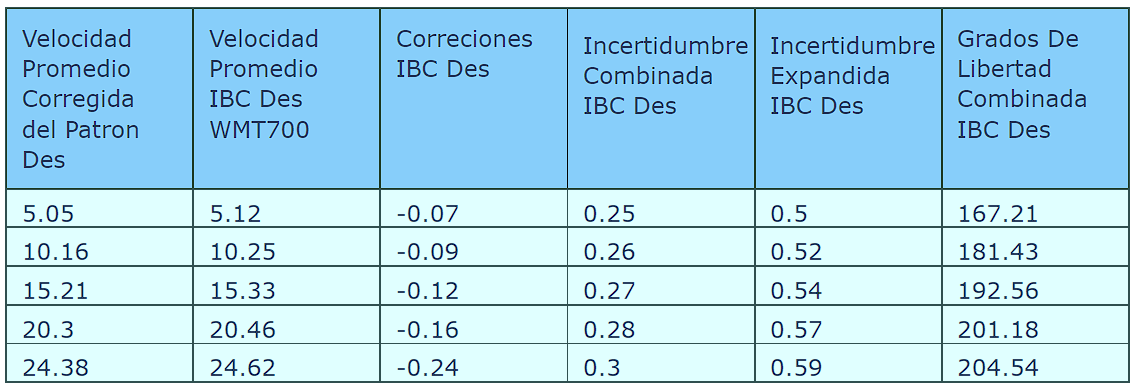
\includegraphics[width=\textwidth]{Figuras/resultados/calibracion/WMT700/tablaVaisalaCalibDes.png}}
%     \end{minipage}  
%     \caption{En (a) se muestra ...y en (b) se observa ... .}
%     \label{fig:vaisalaResultCalibDes}
% \end{figure} 
%-------------------
% Cálculo del factor de bloqueo medición 1
% Sensor Delta OHM

% Primera área (Soporte): 30 cm x 7 cm = 210 cm²
% Segunda área (Sensor): 10 cm x 15 cm = 150 cm²

% Área total en cm²: 210 cm² + 150 cm² = 360 cm²

% convertir a metros cuadrados:
% 360 cm² = 0.036 m²


% Area del patrón
% Primera área (Soporte): 27.5 cm x 8 cm = 220 cm²
% Segunda área (SensorCuernos): 19 cm x 1.5 cm = 28.5 cm²

% Área total en cm²: 28.5 (cm²)*3 + 220 cm² =  305 cm²

% convertir a metros cuadrados:
% 305 cm² = 0.0305 m²


% Entendido, los diámetros de extremo a extremo de la elipse del túnel de viento son 119 cm y 60 cm. Vamos a calcular el área total de la sección transversal de la elipse en metros cuadrados.

% $Area=\pi × radio_mayor × radio_ menor$
% Área = 3.14 x (120/2)x(61/2) = 0.5749 m2

% Factor de Bloqueo DeltaOhm = 0.036/0.5749 = 0.0626
% Factor de Bloqueo Vaisala = 0.0305/0.5749 = 0.05305
% Aca se muestran los resultados de la calibracion del sistema.

% Sistema versatil

% Hacer pruebas con una rampa, y una lineallist